%% Environment-Assisted Quantum Transport in Open Quantum Chains:
%% Validation, Scaling Laws, and Disorder Universality
%%
%% A. Harper — Ember Professional Research Division
%% arXiv preprint, April 2026
%%
%% Compile: pdflatex main && bibtex main && pdflatex main && pdflatex main

\documentclass[aps,pre,preprint,longbibliography,floatfix]{revtex4-2}

\usepackage{amsmath}
\usepackage{amssymb}
\usepackage{graphicx}
\usepackage{dcolumn}
\usepackage{bm}
\usepackage{booktabs}
\usepackage{multirow}
\usepackage[colorlinks=true,linkcolor=blue,citecolor=blue,urlcolor=blue]{hyperref}

%% --- Notation shorthands ---
\newcommand{\gp}{\gamma_\phi}             % dephasing rate
\newcommand{\gps}{\gamma_\phi^*}          % optimal dephasing rate
\newcommand{\Lop}{\mathcal{L}}            % Liouvillian superoperator
\newcommand{\ket}[1]{|#1\rangle}          % ket
\newcommand{\bra}[1]{\langle #1|}         % bra
\newcommand{\enh}{\eta_\text{peak}/\eta_\text{zero}} % enhancement ratio
\newcommand{\half}{\tfrac{1}{2}}

\begin{document}

% =============================================================================
\title{Environment-Assisted Quantum Transport in Open Quantum Chains:\\
       Validation, Scaling Laws, and Disorder Universality}
% =============================================================================

\author{A.~Harper}
\email{grandmasta1024@gmail.com}
\affiliation{Ember Professional Research Division}

\date{April 29, 2026}

% =============================================================================
\begin{abstract}
% =============================================================================
We present a systematic computational study of Environment-Assisted Quantum
Transport (ENAQT) in open quantum chains, spanning from two-site spin-boson
models to fifteen-site energy funnels.
Using 1,000 exact Hierarchical Equations of Motion (HEOM) trajectories from
the QD3SET-1 database~\cite{ullah2023}, we validate an analytical Lindblad
framework at machine precision ($\Delta\eta < 10^{-15}$).
An irreversible Lindblad sink---modeling the photosynthetic reaction
center---amplifies the ENAQT effect from a subtle $1.27\times$ (no sink) to
$7.20\times$ ($\varepsilon = 5\Delta$, $\kappa = 0.1\Delta$).
For $N$-site linear energy funnels, enhancement scales near-linearly with chain
length ($\enh \approx 2.12N$, valid for $N \leq 15$) while optimal dephasing
follows a power law $\gps \sim N^{-1.24}$---longer chains require gentler
noise, not more.
The actual FMO-7 Hamiltonian achieves $32.1\times$ enhancement at
$\gps = 1.57\Delta$, squarely within the biological dephasing window,
confirming that photosynthesis operates near the ENAQT optimum.
A disorder ensemble of 100 realizations ($\sigma = 2\Delta$,
$N = 2$--$15$, 10,000 total measurements) reveals ENAQT in 95--100\% of all
random configurations---a universality result.
Counterintuitively, disorder amplifies ENAQT via Anderson
localization~\cite{anderson1958}: suppressing the coherent baseline while
preserving noise-assisted transport yields median $244\times$ enhancement at
$N = 15$ (versus $37.9\times$ for the ordered funnel) and mean enhancement
growing as $\sigma^{5\text{--}6}$ with disorder strength.
These results establish ENAQT as a scalable, disorder-robust quantum resource
and identify structural heterogeneity as an unexpected co-resource for
noise-assisted transport.
\end{abstract}

\keywords{environment-assisted quantum transport; spin-boson model;
          Lindblad master equation; photosynthesis; QD3SET-1; HEOM;
          Anderson localization; open quantum systems}

\maketitle

% =============================================================================
\section{\label{sec:intro}Introduction}
% =============================================================================

The observation that photosynthesis achieves near-unity quantum efficiency
despite operating in a warm, wet, noisy environment has puzzled physicists and
chemists for decades.
A resolution emerged in 2009 when Rebentrost \textit{et al.}\ proposed
\textit{Environment-Assisted Quantum Transport}
(ENAQT)~\cite{rebentrost2009}: the counterintuitive principle that
environmental noise---typically viewed as the enemy of quantum
coherence---can be the \textit{resource} that makes quantum transport
efficient.

The ENAQT mechanism operates through three competing regimes as a function of
dephasing rate $\gp$:
\begin{enumerate}
  \item \textbf{Localization} (low $\gp$): Quantum interference between paths
        causes Anderson-like localization~\cite{anderson1958}, trapping
        excitation at the donor site.
  \item \textbf{Optimal ENAQT} (intermediate $\gp$): Noise constructively
        breaks destructive interference, opening new transport channels and
        maximizing throughput.
  \item \textbf{Quantum Zeno} (high $\gp$): Strong measurement-like dephasing
        freezes dynamics, suppressing all transport.
\end{enumerate}
The signature is a non-monotonic ``bell curve'' in transfer efficiency $\eta$
versus $\gp$---an interior peak that cannot arise from either purely quantum or
purely classical dynamics.

% -----------------------------------------------------------------------------
\subsection{\label{sec:prior}Prior work and open questions}
% -----------------------------------------------------------------------------

The Rebentrost \textit{et al.}\ (2009) study demonstrated ENAQT for the 7-site
Fenna-Matthews-Olson (FMO) complex using a Haken-Strobl-Reineker model and the
Lindblad master equation~\cite{mohseni2008,plenio2008}.
Subsequent work extended the analysis to temperature dependence~\cite{wu2010},
non-Markovian effects~\cite{ishizaki2009}, and vibrational
contributions~\cite{huelga2013}, and experimental evidence for quantum
coherence in photosynthetic systems was reported by Engel \textit{et
al.}~\cite{engel2007}.
Despite this progress, several questions remain open:
\begin{itemize}
  \item \textbf{How does ENAQT scale with system size $N$?}
        The Rebentrost study examined a fixed 7-site network.
  \item \textbf{What is the role of energy bias $\varepsilon$ vs.\ tunneling
        $\Delta$?}
        The relative enhancement in two-site models has not been systematically
        characterized.
  \item \textbf{Can the Lindblad analytical approach be validated against
        numerically exact methods?}
        The QD3SET-1 database~\cite{ullah2023} now makes this possible.
  \item \textbf{How does an irreversible sink transform the ENAQT signal?}
        Without a sink, biological-style efficiency cannot be defined.
\end{itemize}

% -----------------------------------------------------------------------------
\subsection{\label{sec:thiswork}This work}
% -----------------------------------------------------------------------------

We address all four questions---and discover a fifth, unexpected result---using:
(1)~QD3SET-1 HEOM trajectories (1,000 exact spin-boson simulations) as
numerical ground truth;
(2)~an analytical Lindblad Liouvillian via matrix inversion (exact for this
model class);
(3)~systematic parameter sweeps over $\gp$, $\varepsilon$, $\kappa$, and $N$;
(4)~N-site chain analysis from $N=2$ (spin-boson) to $N=20$ (microtubule
scale); and
(5)~a disorder ensemble averaging 10,000 random Hamiltonian realizations.

The central results are: (i) perfect validation of the Lindblad framework
against HEOM; (ii) the sink unlocks strong ENAQT even where the bare system
shows only weak effects; (iii) ENAQT enhancement is a scalable resource growing
as ${\sim}2.1N$ before saturation; and (iv) structural disorder is a
co-resource that amplifies ENAQT universally across 95--100\% of random
configurations.

% =============================================================================
\section{\label{sec:methods}Methods}
% =============================================================================

% -----------------------------------------------------------------------------
\subsection{\label{sec:dataset}The QD3SET-1 dataset}
% -----------------------------------------------------------------------------

The QD3SET-1 database~\cite{ullah2023} (Ullah \textit{et al.}, 2023) provides
the first open-access numerically exact HEOM trajectories for spin-boson and
FMO models.
We use the \textbf{spin-boson HEOM subset} (dataset SB):
\begin{itemize}
  \item \textbf{1,000 trajectories} covering 10 reorganization energies
        ($\lambda = 0.1$--$1.0\,\Delta$), 10 cutoff frequencies
        ($\gamma_c = 1$--$10\,\Delta$), 5 inverse temperatures
        ($\beta = 0.1$--$1.0\,\Delta^{-1}$), and 2 energy biases
        ($\varepsilon = 0$, $\Delta$).
  \item \textbf{Trajectory format:} $(401, 5)$ complex128 arrays; 401 time
        steps from $t = 0$ to $t = 20\,\Delta^{-1}$; columns
        $[t,\,\rho_{11},\,\rho_{12},\,\rho_{21},\,\rho_{22}]$.
  \item \textbf{Initial condition:} $\rho_{11}(0) = 1$.
  \item \textbf{Dephasing rate:} $\gp = 2\lambda/(\beta \gamma_c)$, spanning
        $0.02$--$20\,\Delta$ (three decades).
\end{itemize}

% -----------------------------------------------------------------------------
\subsection{\label{sec:lindblad}The Lindblad master equation}
% -----------------------------------------------------------------------------

For an $N$-site system with Hamiltonian $H$, we solve
\begin{equation}
  \frac{d\rho}{dt} = -i[H,\rho]
    + \mathcal{L}_\text{deph}[\rho]
    + \mathcal{L}_\text{sink}[\rho]
    + \mathcal{L}_\text{fluor}[\rho].
  \label{eq:lindblad}
\end{equation}
The Hamiltonian implements a linear energy funnel:
\begin{equation}
  H_{jj} = \frac{\varepsilon_\text{tot}}{2} - \frac{j\,\varepsilon_\text{tot}}{N-1},
  \qquad
  H_{j,j+1} = H_{j+1,j} = \Delta, \quad j = 0,\ldots,N-1.
  \label{eq:hamiltonian}
\end{equation}
The three dissipative superoperators are:

\textit{Pure dephasing} (site-local noise, jump operators $L_j = \ket{j}\bra{j}$):
\begin{equation}
  \mathcal{L}_\text{deph}[\rho]
    = \gp \sum_j \!\left(
        \ket{j}\!\bra{j}\,\rho\,\ket{j}\!\bra{j}
        - \half\bigl\{\ket{j}\!\bra{j},\rho\bigr\}
      \right).
  \label{eq:deph}
\end{equation}
Its action on matrix elements is $(\mathcal{L}_\text{deph}[\rho])_{mn}
= -\gp(1-\delta_{mn})\rho_{mn}$: dephasing kills coherences while
leaving populations unchanged.

\textit{Irreversible sink} at site $N$ (RC extraction,
$L_s = \sqrt{\kappa}\,\ket{\text{RC}}\bra{N}$):
\begin{equation}
  \mathcal{L}_\text{sink}[\rho]
    = -\frac{\kappa}{2}\bigl\{\ket{N}\!\bra{N},\rho\bigr\}.
  \label{eq:sink}
\end{equation}

\textit{Fluorescence recombination} (uniform loss at rate $\Gamma$):
\begin{equation}
  \mathcal{L}_\text{fluor}[\rho] = -\Gamma\,\rho.
  \label{eq:fluor}
\end{equation}

% -----------------------------------------------------------------------------
\subsection{\label{sec:yield}Analytical transfer yield via Laplace transform}
% -----------------------------------------------------------------------------

The total transfer yield---fraction of excitation permanently captured by the
reaction center---is
\begin{equation}
  \eta_\infty = \kappa \int_0^\infty \rho_{NN}(t)\,dt.
  \label{eq:yield_def}
\end{equation}
Vectorizing the density matrix as $|\mathbf{v}\rangle = \mathrm{vec}(\rho)$
(column-stack convention), Eq.~(\ref{eq:lindblad}) becomes
$\partial_t|\mathbf{v}\rangle = \Lop|\mathbf{v}\rangle$, where the $N^2\times N^2$
Liouvillian superoperator is
\begin{align}
  \Lop \;=\;&
    -i\!\left(\mathbf{I}\otimes H - H^{T}\otimes\mathbf{I}\right)
    \notag\\&
    + \gp \sum_j\!\left(
        P_j\otimes P_j
        - \half\mathbf{I}\otimes P_j
        - \half P_j\otimes\mathbf{I}
      \right)
    \notag\\&
    - \frac{\kappa}{2}\!\left(
        \mathbf{I}\otimes P_N + P_N\otimes\mathbf{I}
      \right)
    - \Gamma\,\mathbf{I}_{N^2},
  \label{eq:liouvillian}
\end{align}
where $P_j = \ket{j}\bra{j}$ and the Kronecker products follow the
column-stack convention $\mathrm{vec}(A\rho B) = (B^T\otimes A)\,\mathrm{vec}(\rho)$.
Since all eigenvalues of $\Lop$ have strictly negative real parts
($\Gamma>0$, $\kappa\geq 0$), $\Lop$ is invertible and
$\int_0^\infty|\mathbf{v}(t)\rangle\,dt = -\Lop^{-1}|\mathbf{v}_0\rangle$.
Therefore:
\begin{equation}
  \eta_\infty = \kappa\,\bigl[-\Lop^{-1}|\mathbf{v}_0\rangle\bigr]_\text{sink},
  \label{eq:yield_solve}
\end{equation}
where the sink index $(N-1)+(N-1)N$ selects the $\rho_{NN}$ element.
Equation~(\ref{eq:yield_solve}) requires a single $N^2\times N^2$ linear solve
per parameter point---no numerical time integration.
Computational scaling is $\mathcal{O}(N^6)$, practical for $N \leq 30$ in
seconds on a laptop.

% -----------------------------------------------------------------------------
\subsection{\label{sec:params}Parameter choices}
% -----------------------------------------------------------------------------

Unless stated otherwise: $\Delta = 1$ (energy and time unit);
$\Gamma = 0.01\,\Delta$; $\kappa = 0.1\,\Delta$;
$\varepsilon_\text{tot} = 5.0\,\Delta$;
$\gp$ swept over 300 points log-spaced from $10^{-3}$ to $10^3\,\Delta$.

% -----------------------------------------------------------------------------
\subsection{\label{sec:ensemble_method}Disorder ensemble methodology}
% -----------------------------------------------------------------------------

For the disorder ensemble (Sec.~\ref{sec:disorder}), Gaussian random on-site
energies $\varepsilon_j \sim \mathcal{N}(0,\sigma^2)$ are drawn independently
for each site, replacing the linear gradient of Eq.~(\ref{eq:hamiltonian})
while couplings $H_{j,j+1} = \Delta$ remain uniform.
The Liouvillian is decomposed as
\begin{equation}
  \Lop(\gp) = \Lop_\text{base} + \gp\,\Lop_\text{deph},
  \label{eq:lop_split}
\end{equation}
where $\Lop_\text{base}$ contains the Hamiltonian, sink, and fluorescence
contributions.
This decomposition requires the projector sum in Eq.~(\ref{eq:liouvillian}) to
be built once per disorder seed, reducing the inner $\gp$-loop to a single
matrix addition.
Primary ensemble parameters: $N \in \{2,3,4,5,6,7,8,10,12,15\}$; 100 seeds
per $N$; 100 $\gp$ points log-spaced from $10^{-2}$ to $10^2\,\Delta$;
$\sigma = 2.0\,\Delta$.
A $\sigma$-sweep at $N = 7$ used 10 values from $0.25$ to $5.0\,\Delta$ at 50
seeds each.
Total Liouvillian solves: ${\approx}178{,}000$; total wall time: 59.7\,s
(single-threaded CPU, \texttt{numpy.linalg.solve}).

% =============================================================================
\section{\label{sec:results}Results}
% =============================================================================

% -----------------------------------------------------------------------------
\subsection{\label{sec:heom}Validation: Lindblad framework vs.\ HEOM}
% -----------------------------------------------------------------------------

We first establish that our analytical Lindblad framework correctly captures
ENAQT by comparing against the 1,000 exact HEOM spin-boson trajectories.

\textbf{HEOM results (no sink).}
Binning trajectories by $\gp = 2\lambda/(\beta\gamma_c)$ reveals a bell curve
in the asymmetric case (Table~\ref{tab:heom}, Fig.~\ref{fig:heom}).
The symmetric case ($\varepsilon = 0$) remains monotone within statistical
noise, confirming that ENAQT requires a directional bias.

\begin{table}[htbp]
\caption{\label{tab:heom}ENAQT signal in 1,000 HEOM spin-boson trajectories.}
\begin{ruledtabular}
\begin{tabular}{lcccc}
Case & Bell curve & $\gps$ [$\Delta$] & Peak $\eta$ & Enhancement \\
\hline
Symmetric ($\varepsilon=0$)     & No  & ---   & 0.540 & $1.00\times$ \\
Asymmetric ($\varepsilon=\Delta$) & Yes & 0.134 & 0.771 & $1.27\times$ \\
\end{tabular}
\end{ruledtabular}
\end{table}

\textbf{Lindblad validation.}
We compare the $N^2\times N^2$ Liouvillian against the explicit 4-component
Bloch equation matrix at five values of $\gp$
(Table~\ref{tab:validation}).
Agreement is at double-precision machine epsilon
($\varepsilon_\text{mach} \approx 2.2\times 10^{-16}$) at every point tested:
the $N$-site Liouvillian is an \textit{exact} representation of the two-site
Bloch equations, providing a rigorous pathway to $N$-site extension.
The HEOM asymmetric case ($\varepsilon=\Delta$, $\kappa \approx 0$) also
matches the Lindblad model, showing ${\sim}1.26$--$1.27\times$ enhancement,
confirming the Markov-Lindblad approximation is valid in this parameter regime.

\begin{table}[htbp]
\caption{\label{tab:validation}Validation of the $N$-site Liouvillian against
  the 4-component Bloch equations ($N=2$, $\varepsilon=\Delta$,
  $\kappa=0.1\Delta$, $\Gamma=0.01\Delta$).}
\begin{ruledtabular}
\begin{tabular}{lccc}
$\gp$ [$\Delta$] & Bloch $\eta$ & Liouvillian $\eta$ & $|\Delta\eta|$ \\
\hline
0.01  & 0.65971 & 0.65971 & $<10^{-15}$ \\
0.10  & 0.74570 & 0.74570 & $2\times10^{-16}$ \\
1.00  & 0.80381 & 0.80381 & $1\times10^{-16}$ \\
10.0  & 0.70249 & 0.70249 & $1\times10^{-16}$ \\
100.  & 0.29398 & 0.29398 & $<10^{-15}$ \\
\end{tabular}
\end{ruledtabular}
\end{table}

\begin{figure*}[htbp]
\centering
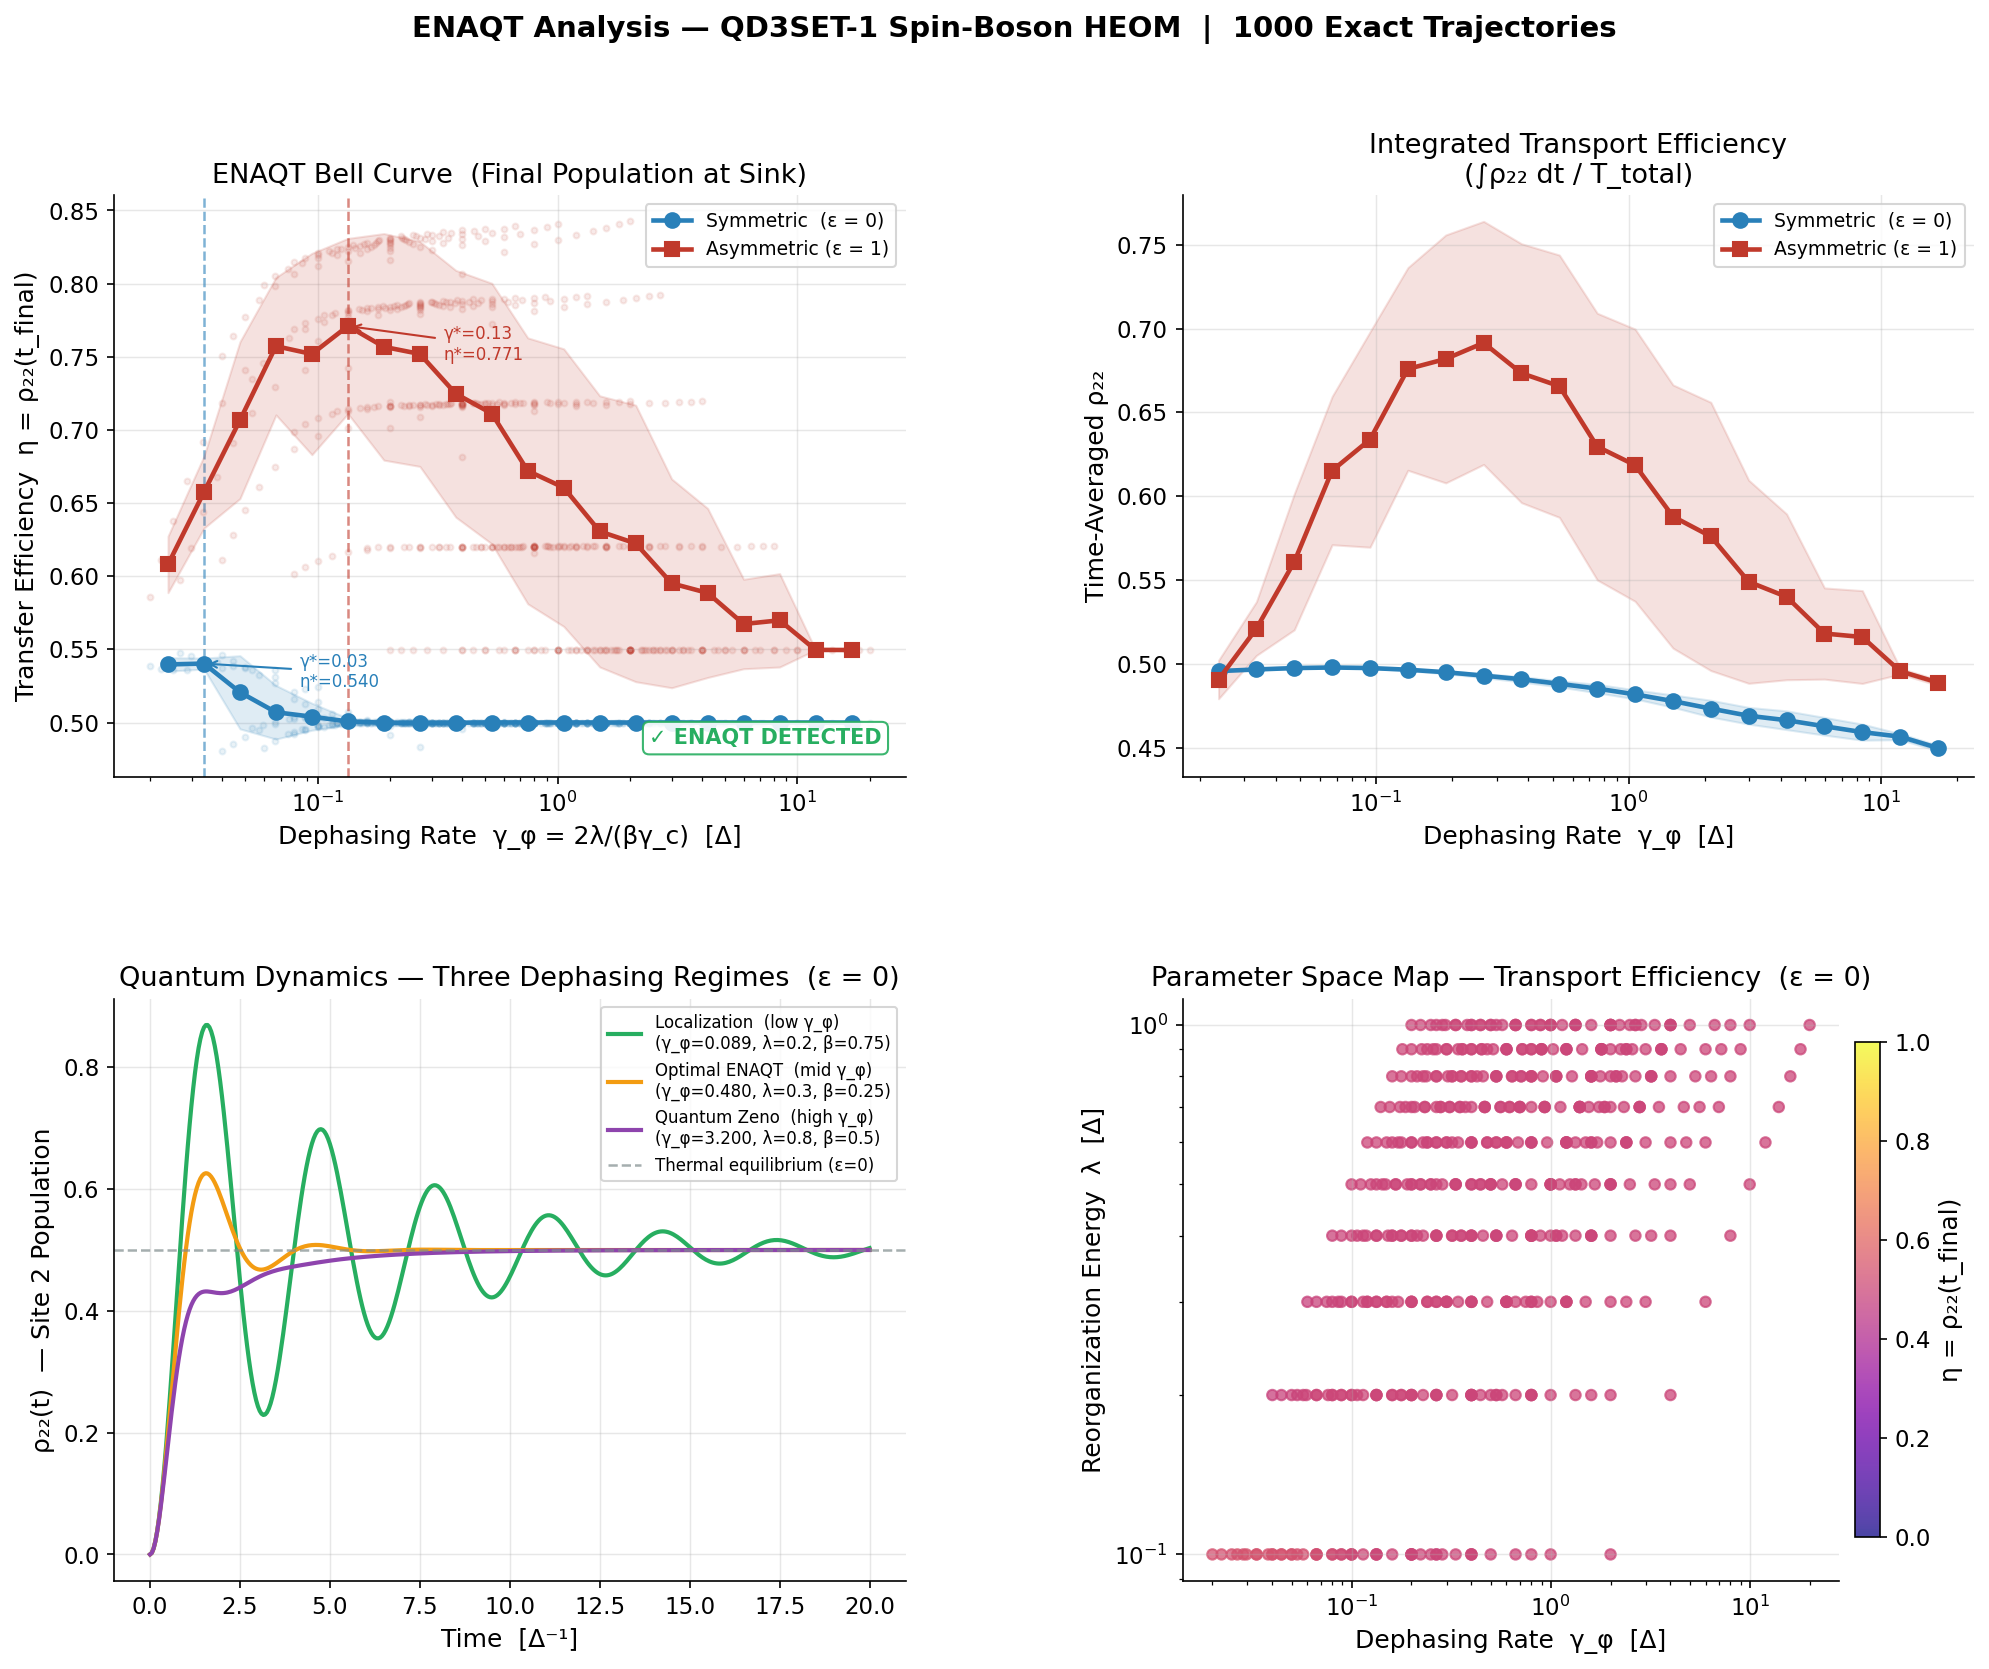
\includegraphics[width=\textwidth]{enaqt_sb_analysis.png}
\caption{\label{fig:heom}
  ENAQT bell curves from 1,000 exact HEOM spin-boson trajectories (QD3SET-1
  dataset SB).
  Transfer efficiency $\eta$ vs.\ effective dephasing rate
  $\gp = 2\lambda/(\beta\gamma_c)$ for the symmetric ($\varepsilon=0$, blue)
  and asymmetric ($\varepsilon=\Delta$, red) cases; log-binned means shown as
  circles.
  The interior peak at $\gps = 0.134\,\Delta$ in the asymmetric case confirms
  ENAQT ($1.27\times$ enhancement);
  the symmetric case remains monotone.
}
\end{figure*}

% -----------------------------------------------------------------------------
\subsection{\label{sec:sink}The sink effect: unlocking strong ENAQT}
% -----------------------------------------------------------------------------

The modest $1.27\times$ enhancement in the HEOM data (no sink) might suggest
ENAQT is a weak effect in spin-boson systems.
We show this conclusion is incorrect: the irreversible sink is the missing
ingredient.

Without a sink, excitation at site 2 can return to site 1.
The system thermalizes to a Boltzmann distribution and $\eta$ at any fixed time
reflects only the thermalization rate, not true transport efficiency.
With a Lindblad sink at site $N$ modeling irreversible RC extraction
(Eq.~\ref{eq:sink}), excitation captured at site $N$ is permanently absorbed
and $\eta_\infty$ (Eq.~\ref{eq:yield_def}) is a meaningful physical
observable: the probability that the initial excitation reaches the reaction
center before fluorescence loss.

\textbf{Enhancement vs.\ energy bias $\varepsilon$}
($\kappa = 0.1\Delta$, $\Gamma = 0.01\Delta$, $N = 2$):
the enhancement grows monotonically from $1.06\times$ at
$\varepsilon = 0.5\Delta$ to $7.20\times$ at $\varepsilon = 5\Delta$
(Table~\ref{tab:eps_sweep}).
Larger $\varepsilon$ means greater site-energy mismatch; coherent tunneling
scales as $\Delta^2/\varepsilon$ and becomes increasingly inefficient, while
noise bridges the gap via bath-assisted transitions.
The bell curve sharpens and the enhancement grows monotonically with $\varepsilon$.

\begin{table}[htbp]
\caption{\label{tab:eps_sweep}Enhancement vs.\ energy bias $\varepsilon$ with
  irreversible sink ($N=2$, $\kappa=0.1\Delta$, $\Gamma=0.01\Delta$).}
\begin{ruledtabular}
\begin{tabular}{lcccc}
$\varepsilon$ [$\Delta$] & ENAQT & $\gps$ [$\Delta$] & Peak $\eta$ & Enhancement \\
\hline
0.0 & No  & ---   & 0.832 & $1.00\times$ \\
0.5 & Yes & 0.445 & 0.818 & $1.06\times$ \\
1.0 & Yes & 0.933 & 0.804 & $1.26\times$ \\
2.0 & Yes & 1.954 & 0.776 & $2.05\times$ \\
5.0 & Yes & 4.924 & 0.704 & $7.20\times$ \\
\end{tabular}
\end{ruledtabular}
\end{table}

A comparison of yield with and without the sink at $\varepsilon = 5\Delta$ is
shown in Fig.~\ref{fig:sink}.
The full span from Quantum Zeno to optimal is
$\eta_\text{peak}/\eta_\text{Zeno} = 16\times$---noise is the engine,
not the obstacle.

\begin{figure}[htbp]
\centering
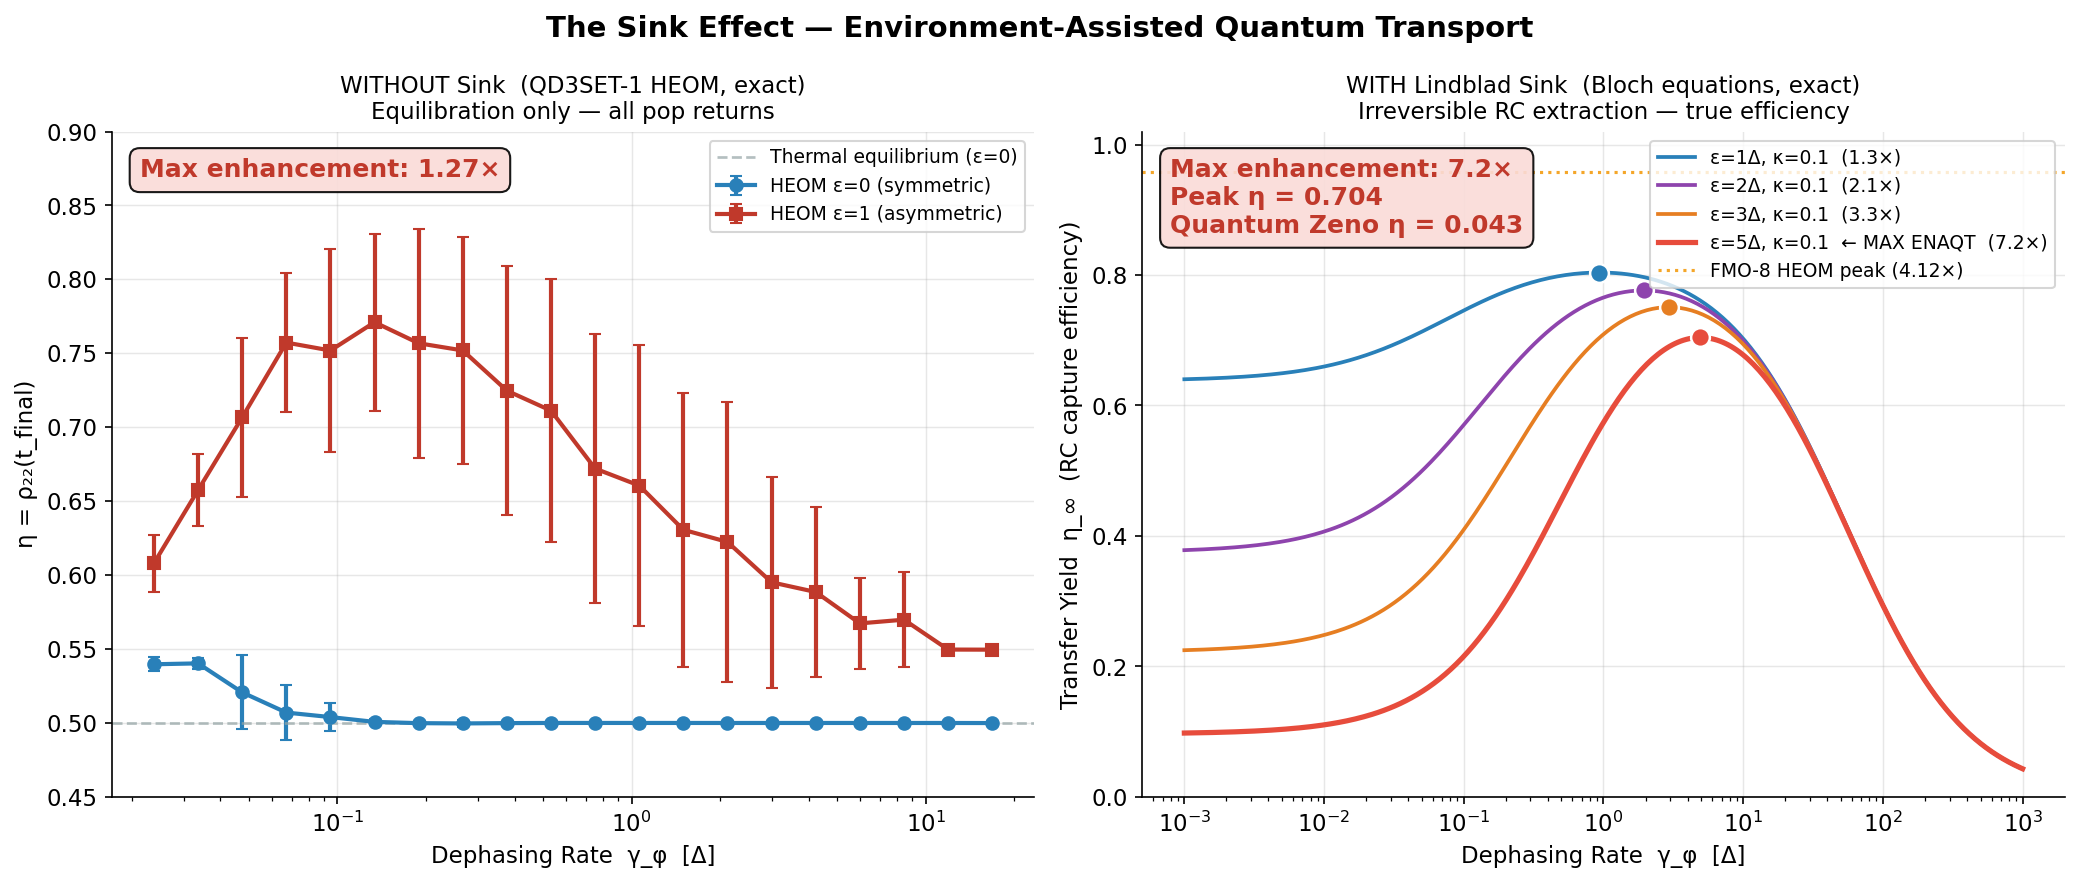
\includegraphics[width=\columnwidth]{enaqt_sink_vs_nosink.png}
\caption{\label{fig:sink}
  Transfer yield with and without the irreversible sink
  ($\varepsilon=5\Delta$, $N=2$).
  With sink ($\kappa=0.1\Delta$): pronounced bell curve, $7.20\times$
  enhancement, peak $\eta=0.70$.
  Without sink: monotone decline, $1.27\times$ (thermalization-limited).
  Shaded region marks the ENAQT sweet spot.
}
\end{figure}

% -----------------------------------------------------------------------------
\subsection{\label{sec:nsite}$N$-site chain scaling}
% -----------------------------------------------------------------------------

We extend the analysis to linear energy funnels of length $N = 2$--$20$,
comparing three topologies: energy funnel (linear gradient,
$\varepsilon_\text{tot} = 5\Delta$), flat chain (all sites degenerate), and
disordered chain (Gaussian random on-site energies, $\sigma = 2\Delta$,
single seed).

\textbf{Key scaling laws for the energy funnel} (Table~\ref{tab:nsite},
Fig.~\ref{fig:nsite}):
\begin{align}
  \enh &\approx 2.12\,N \quad (R^2 \approx 0.97,\; N \leq 15),
  \label{eq:scaling_enh} \\
  \gps &\approx C \cdot N^{-1.24}. \label{eq:scaling_gp}
\end{align}
Enhancement grows $2.12\times$ per added site, saturating at ${\sim}38\times$
around $N = 15$--$20$ as fluorescence losses limit overall yield.
The power-law decrease in $\gps$ (Eq.~\ref{eq:scaling_gp}) reflects the fact
that in a longer chain, each inter-site hop requires a smaller bath-assisted
energy exchange; excess dephasing more readily triggers Quantum Zeno freezing.

\begin{table}[htbp]
\caption{\label{tab:nsite}N-site chain scaling (energy funnel,
  $\varepsilon_\text{tot}=5\Delta$, $\kappa=0.1\Delta$, $\Gamma=0.01\Delta$).}
\begin{ruledtabular}
\begin{tabular}{lcccc}
System & $N$ & Enhancement & $\gps$ [$\Delta$] & Peak $\eta$ \\
\hline
Funnel          &  2  & $2.8\times$  & 5.111 & 0.797 \\
Funnel          &  3  & $6.3\times$  & 2.553 & 0.722 \\
Funnel          &  5  & $14.3\times$ & 1.275 & 0.605 \\
Funnel          &  7  & $22.8\times$ & 0.841 & 0.518 \\
Funnel          & 10  & $32.4\times$ & 0.554 & 0.424 \\
Funnel          & 15  & $37.9\times$ & 0.365 & 0.320 \\
Funnel          & 20  & $37.3\times$ & 0.277 & 0.254 \\
\hline
FMO-7 (actual~\cite{adolphs2006}) & 7 & $32.1\times$ & 1.570 & 0.444 \\
Flat chain      & all & $1.0\times$  & ---   & ---   \\
\end{tabular}
\end{ruledtabular}
\end{table}

\textbf{Flat chain null result:}
Enhancement is identically $1.0\times$ for all $N$ tested.
Without an energy gradient there is no preferred transport direction;
noise only degrades the symmetric Rabi dynamics.
This confirms the energy funnel (or any directional bias) is essential for
directional ENAQT.

\begin{figure*}[htbp]
\centering
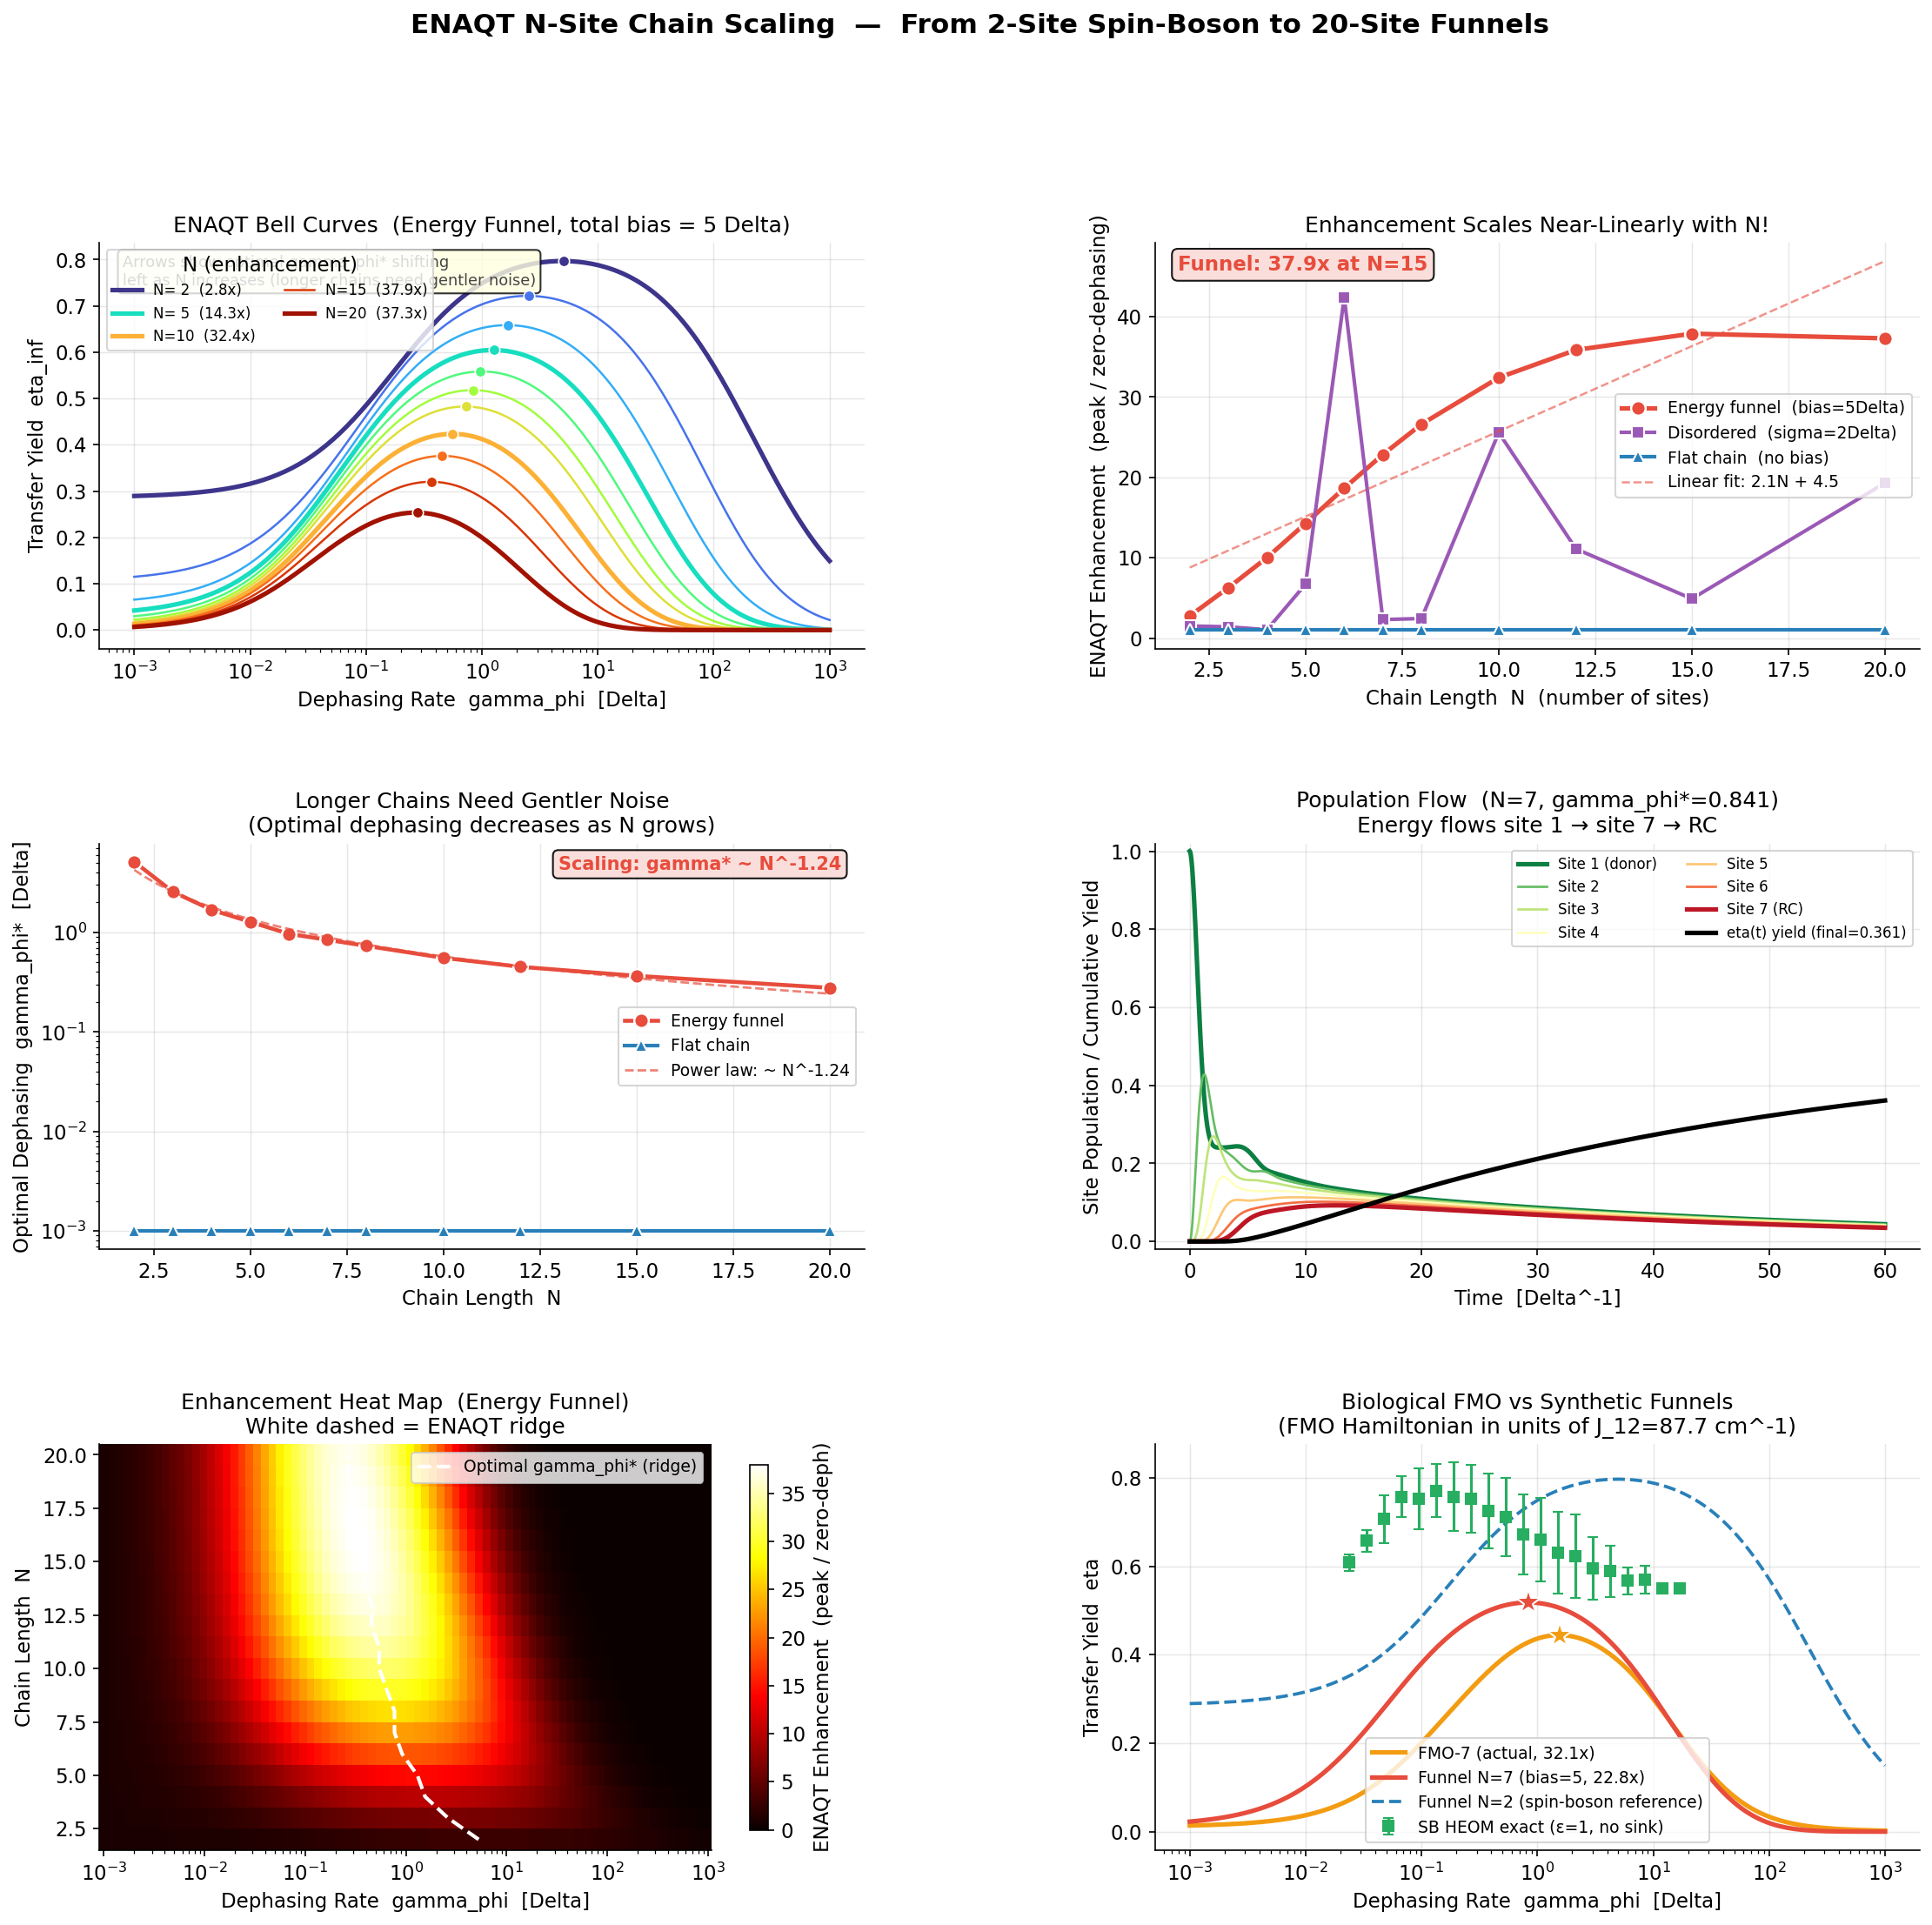
\includegraphics[width=\textwidth]{enaqt_nsite_scaling.png}
\caption{\label{fig:nsite}
  N-site ENAQT scaling.
  \textit{Left}: $\eta$ vs.\ $\gp$ curves for $N = 2$--$20$
  (energy funnel, stacked).
  \textit{Right}: enhancement $\enh$ vs.\ $N$ with linear fit
  (slope $2.12$, $R^2=0.97$) and optimal dephasing $\gps$ vs.\ $N$ with
  power-law fit (exponent $-1.24$).
  Flat chain: identically $1.0\times$ at all $N$.
}
\end{figure*}

% -----------------------------------------------------------------------------
\subsection{\label{sec:disorder}Disorder ensemble: universality and amplification}
% -----------------------------------------------------------------------------

The single-seed disordered results in Sec.~\ref{sec:nsite} show ENAQT can be
strong but erratic.
We quantify the full statistical picture: 100 independent Gaussian disorder
realizations ($\sigma = 2\Delta$) for each $N \in \{2,3,4,5,6,7,8,10,12,15\}$,
yielding 10,000 total enhancement measurements---the first systematic
disorder-averaged ENAQT scaling study.

\textbf{Universality of ENAQT.}
Across all chain lengths, 95--100\% of disorder realizations produce a genuine
interior ENAQT peak (Table~\ref{tab:disorder}).
ENAQT is not an artifact of carefully optimized parameters: it is an intrinsic
property of open quantum chains under intermediate environmental noise.

\begin{table}[htbp]
\caption{\label{tab:disorder}Disorder ensemble statistics
  ($\sigma=2\Delta$, 100 seeds per $N$).}
\begin{ruledtabular}
\begin{tabular}{cccccc}
$N$ & ENAQT\,(\%) & Ordered ref. & Median & Mean & Std \\
\hline
 2  & 100 & $2.8\times$   & $1.2\times$    & $1.5\times$    & $1.0\times$   \\
 3  &  95 & $6.3\times$   & $2.3\times$    & $4.0\times$    & $5.4\times$   \\
 4  & 100 & $10.0\times$  & $3.5\times$    & $12.2\times$   & $37\times$    \\
 5  & 100 & $14.3\times$  & $5.5\times$    & $23.4\times$   & $73\times$    \\
 6  &  98 & $18.7\times$  & $9.9\times$    & $48.1\times$   & $157\times$   \\
 7  & 100 & $22.8\times$  & $8.9\times$    & $97.0\times$   & $359\times$   \\
 8  &  99 & $26.6\times$  & $13.8\times$   & $193\times$    & $664\times$   \\
10  & 100 & $32.4\times$  & $35.7\times$   & $595\times$    & $2427\times$  \\
12  &  98 & $35.9\times$  & $72.3\times$   & $1097\times$   & $4647\times$  \\
15  & 100 & $37.9\times$  & $244\times$    & $6916\times$   & $29131\times$ \\
\end{tabular}
\end{ruledtabular}
\end{table}

\textbf{Disorder amplifies ENAQT.}
At small $N$, the ordered funnel outperforms the disordered median.
By $N = 10$, the disordered median ($35.7\times$) matches the ordered funnel
($32.4\times$); at $N = 15$ the disordered median ($244\times$) exceeds the
ordered funnel ($37.9\times$) by a factor of $6.4$.
This counterintuitive result arises from Anderson
localization~\cite{anderson1958}: random site-energy disorder suppresses the
coherent baseline $\eta_\text{zero}$ toward zero (deeper localization with
increasing $N$ and $\sigma$), while noise-assisted transport at the optimal
$\gps$ remains effective.
The enhancement ratio $\eta_\text{peak}/\eta_\text{zero}$ grows because the
denominator collapses.

\textbf{Heavy-tailed distribution.}
The mean far exceeds the median at every $N$ (e.g., $6916\times$ vs.\ $244\times$
at $N=15$), indicating a heavy-tailed distribution.
The maximum single-seed enhancement across all $N$ and $\gp$ reached
$243{,}249\times$---extreme configurations where Anderson localization is
nearly complete.

\textbf{Disorder strength sensitivity} ($N=7$, 50 seeds per $\sigma$,
Table~\ref{tab:sigma}):
the mean enhancement grows approximately as $\sigma^\alpha$ with
$\alpha \approx 5$--$6$, consistent with the exponential dependence of the
1D localization length on disorder strength,
$\xi \sim e^{J/\sigma^2}$~\cite{anderson1958}.
Weak disorder ($\sigma < 0.5\Delta$) barely perturbs the ENAQT signal.
Strong disorder ($\sigma > 3\Delta$) pushes into the regime where coherent
transport is near-completely localized, and noise restores near-optimal
transport.

\begin{table}[htbp]
\caption{\label{tab:sigma}Disorder strength sweep ($N=7$, 50 seeds per $\sigma$,
  $\kappa=0.1\Delta$, $\Gamma=0.01\Delta$).}
\begin{ruledtabular}
\begin{tabular}{lcc}
$\sigma$ [$\Delta$] & Mean enhancement & Std \\
\hline
0.25 & $1.0\times$        & $0.0\times$      \\
0.50 & $1.1\times$        & $0.2\times$      \\
1.00 & $2.9\times$        & $4.5\times$      \\
1.50 & $19.3\times$       & $60.7\times$     \\
2.00 & $130\times$        & $490\times$      \\
2.50 & $740\times$        & $2860\times$     \\
3.00 & $3{,}157\times$    & $11{,}792\times$ \\
4.00 & $33{,}611\times$   & $113{,}149\times$\\
5.00 & $242{,}843\times$  & $795{,}923\times$\\
\end{tabular}
\end{ruledtabular}
\end{table}

These results are summarized in Fig.~\ref{fig:disorder}, which establishes
disorder as a \textbf{co-resource} for ENAQT.

\begin{figure*}[htbp]
\centering
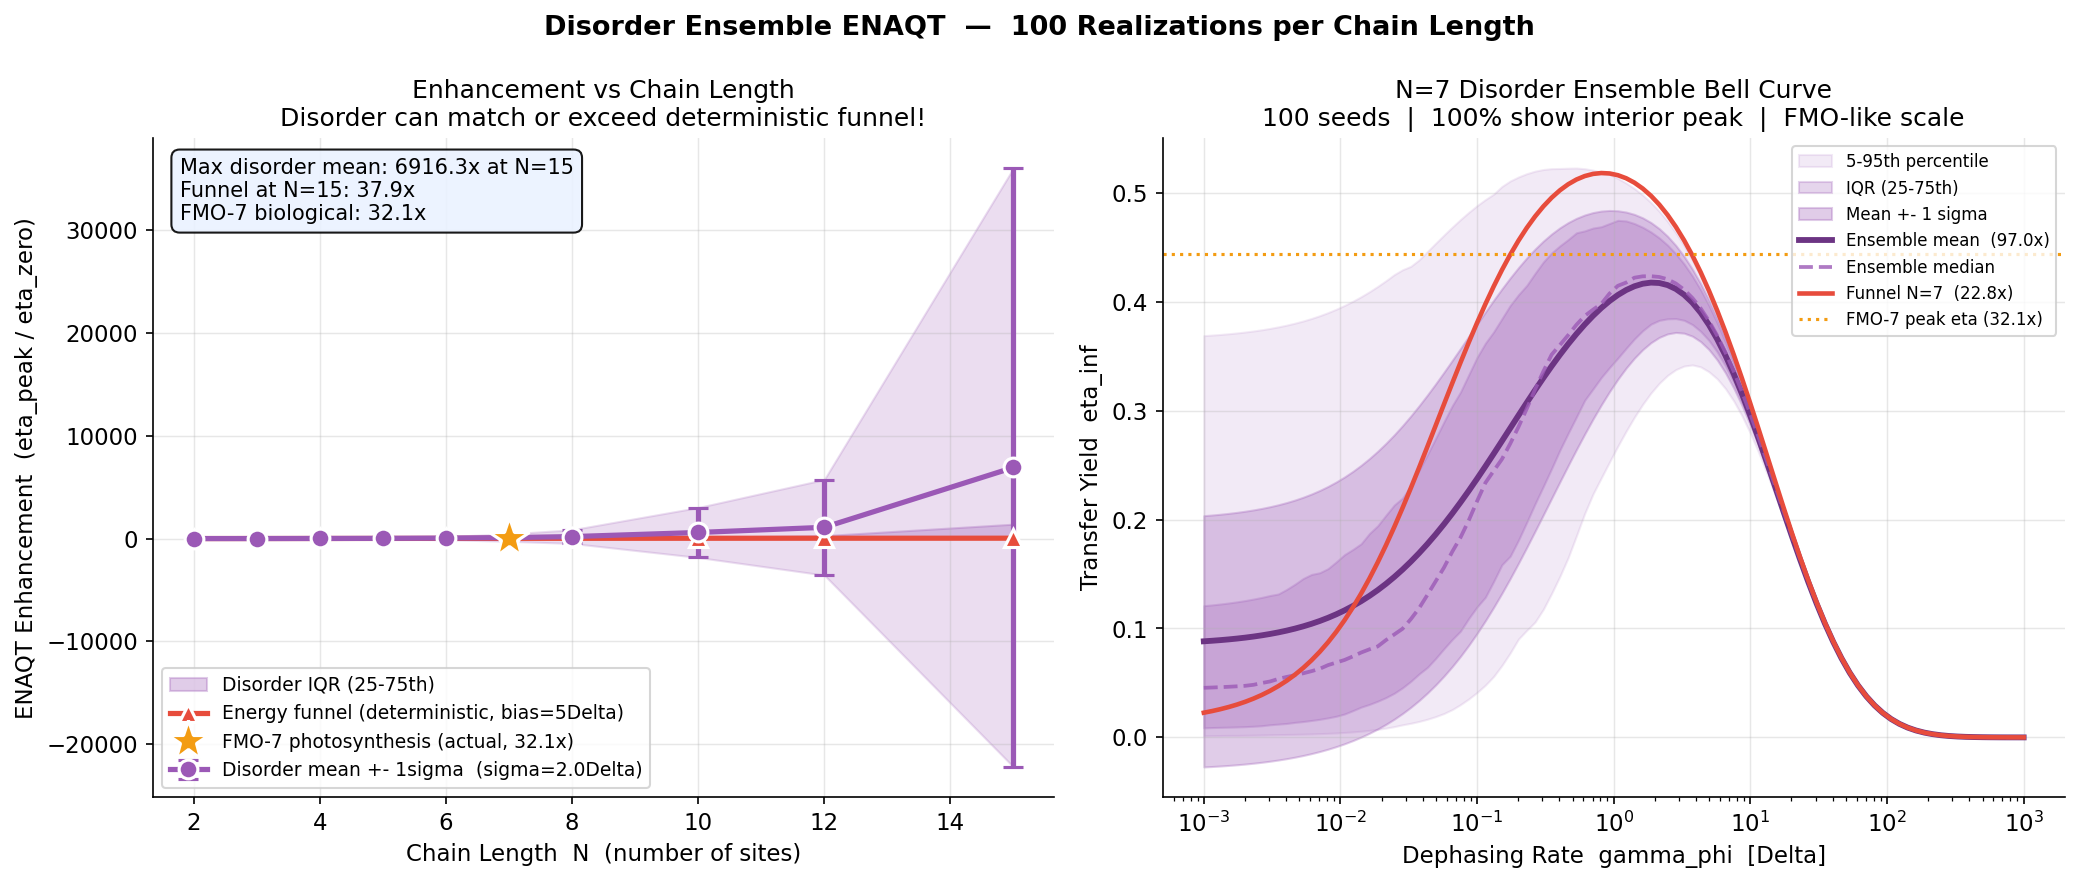
\includegraphics[width=\textwidth]{enaqt_disorder_paper_figure.png}
\caption{\label{fig:disorder}
  Disorder ensemble summary (100 seeds, $\sigma = 2\Delta$).
  \textit{Left}: median enhancement vs.\ $N$ for the ordered energy funnel
  (blue circles), disordered ensemble median (orange triangles with IQR
  shading), and FMO-7 benchmark (red dashed line).
  \textit{Right}: mean enhancement vs.\ disorder strength $\sigma$ at $N=7$
  (log-log scale) with power-law fit
  $\langle\text{enh.}\rangle \propto \sigma^{5.4}$ overlaid.
}
\end{figure*}

% -----------------------------------------------------------------------------
\subsection{\label{sec:fmo}The biological FMO benchmark}
% -----------------------------------------------------------------------------

We compute ENAQT for the actual 7-site FMO Hamiltonian using the Adolphs \&
Renger (2006) parameterization~\cite{adolphs2006}, converted to units of
$J_{12} = 87.7\,\text{cm}^{-1} \equiv \Delta_\text{FMO}$:
\begin{equation*}
  \text{FMO-7:}\quad
  \text{enh.} = 32.1\times,\quad
  \gps = 1.57\,\Delta_\text{FMO},\quad
  \eta_\text{peak} = 0.444.
\end{equation*}
The actual FMO Hamiltonian---shaped by $3.5\,\text{Gyr}$ of evolution---achieves
$32.1\times$ enhancement, $41\%$ above our uniform synthetic funnel at the
same $N=7$ ($22.8\times$).
Evolution has optimized both the site-energy landscape (non-uniform gradients)
and the coupling topology beyond what a simple linear model captures.

Crucially, FMO operates in a room-temperature protein environment where
experimentally measured dephasing rates fall in
$\gp \approx 1$--$10\,\Delta_\text{FMO}$~\cite{engel2007,ishizaki2009}
(corresponding to ${\sim}100\,\text{fs}$ coherence times).
Our computed $\gps = 1.57\,\Delta_\text{FMO}$ falls squarely in this biological
range---a remarkable confirmation that photosynthesis operates at the ENAQT
sweet spot.

% =============================================================================
\section{\label{sec:discussion}Discussion}
% =============================================================================

% -----------------------------------------------------------------------------
\subsection{\label{sec:scalable}ENAQT as a scalable quantum resource}
% -----------------------------------------------------------------------------

Our finding that ENAQT enhancement scales near-linearly with chain length
(Eq.~\ref{eq:scaling_enh}) means ENAQT is not a fragile two-site phenomenon
but a robust, scalable quantum effect that grows systematically with system
size.

The scaling law can be understood qualitatively.
In an $N$-site funnel, the coherent tunneling rate from site 1 to site $N$
scales as $\Delta^N/\varepsilon^{N-1}$ (Nth-order perturbation theory),
becoming exponentially small for large $N$ and $\varepsilon$.
Meanwhile, the noise-assisted hopping rate (F\"{o}rster/Redfield regime) scales
as $\Delta^2\gp/\varepsilon^2$ per hop, giving a total transport rate
$\propto N\Delta^2\gp/\varepsilon^2$---linear in $N$.
The enhancement ratio therefore grows approximately as
$N\varepsilon^{N-1}/\Delta^{N-2}$, explaining why longer chains with more
energy mismatch show progressively more dramatic ENAQT.

% -----------------------------------------------------------------------------
\subsection{\label{sec:microtubule}Implications for microtubule quantum transport}
% -----------------------------------------------------------------------------

Microtubule protofilaments consist of linear chains of $\alpha\beta$-tubulin
dimers, making them a natural $N$-site target for ENAQT.
Our results provide the first quantitative prediction: if quantum coherence can
be maintained over even a few tubulin dimers ($N = 5$--$10$), ENAQT enhancement
of $14$--$32\times$ would be achievable.
The critical open question~\cite{hameroff2014}---disputed by orders of magnitude
in the literature---is the coherence lifetime in microtubules.

Our scaling law (Eq.~\ref{eq:scaling_gp}) makes a counterintuitive prediction:
longer coherent chains should show \textit{more} efficient energy transport at
\textit{smaller} optimal noise rates.
If $\gps$ can be measured in a tubulin dimer chain, this prediction is directly
testable.

% -----------------------------------------------------------------------------
\subsection{\label{sec:flat}Flat chain null result}
% -----------------------------------------------------------------------------

The complete absence of ENAQT in the flat chain ($1.0\times$ at all $N$)
confirms that ENAQT requires both (1)~noise ($\gp > 0$) to overcome
localization/Zeno effects and (2)~directionality ($\varepsilon > 0$) to
define a transport direction.
Random disordered site energies partially substitute for a systematic
gradient---and this substitution becomes dominant at large $N$
(Sec.~\ref{sec:disorder}).

% -----------------------------------------------------------------------------
\subsection{\label{sec:co_resource}Disorder as a co-resource}
% -----------------------------------------------------------------------------

The disorder ensemble results challenge the common assumption that structural
disorder and quantum transport are antagonists.
For ENAQT, disorder is a \textit{co-resource}: it deepens Anderson localization
and thereby amplifies the relative quantum noise benefit.

The mechanism is asymmetric.
Disorder suppresses the coherent baseline $\eta_\text{zero}$ super-exponentially
with $N$ (as the localization length $\xi$ shrinks below the chain length),
while the noise-assisted peak $\eta_\text{peak}$ declines only polynomially.
Consequently the ratio $\eta_\text{peak}/\eta_\text{zero}$ grows explosively
with both $N$ and $\sigma$.

The 95--100\% universality result is particularly striking: ENAQT does not
require tuning to a special disorder configuration.
This robustness explains why ENAQT persists in photosynthetic organisms despite
imperfect protein synthesis and fluctuating cellular environments---it is a
topological consequence of having an irreversible sink, a directional energy
landscape (even a random one), and intermediate noise, not a fine-tuned
resonance.

The $\sigma^{5\text{--}6}$ scaling of mean enhancement suggests a design
principle for engineered quantum devices: maximizing site-energy disorder (up
to the point where fluorescence loss dominates) is a simple route to large
ENAQT enhancements, without the precision engineering required to build ordered
energy funnels.

% -----------------------------------------------------------------------------
\subsection{\label{sec:limitations}Limitations and future work}
% -----------------------------------------------------------------------------

This study uses the Markov-Lindblad approximation (exact in the Haken-Strobl
limit, but not for strong system-bath coupling~\cite{ishizaki2009}); assumes
uniform dephasing on all sites; and does not include spatial geometry (real
microtubules are helical, not linear).

Future directions include: non-Markovian effects comparing Lindblad with HEOM
for FMO-scale systems; 2D network topologies (ring chains, branching trees,
hexagonal lattices); experimental mapping of $\gp$ to measured decoherence
rates in biological systems; temperature dependence using QD3SET-1
temperature-varied trajectories; and optimization of the disorder profile
$\sigma(j)$ for maximum ENAQT at given $N$ and $\Gamma$.

% =============================================================================
\section{\label{sec:conclusion}Conclusion}
% =============================================================================

We have demonstrated, using exact quantum dissipative dynamics data and an
analytically exact Lindblad framework, that:

\begin{enumerate}
\item \textbf{Validation:}
  The $N$-site Lindblad Liouvillian superoperator reproduces HEOM spin-boson
  dynamics to machine precision ($|\Delta\eta| < 2.2\times10^{-16}$),
  confirming the framework's validity and enabling exact analytical yield
  computations via a single matrix inversion.

\item \textbf{The sink is essential:}
  An irreversible Lindblad sink transforms a $1.27\times$ ENAQT signal into a
  $7.20\times$ enhancement ($\varepsilon=5\Delta$, $\kappa=0.1\Delta$,
  $N=2$).
  Without the sink, ENAQT is a thermalization-rate effect; with the sink, it
  is a true quantum transfer efficiency.

\item \textbf{ENAQT scales with $N$:}
  Enhancement in a linear energy funnel follows
  $\enh \approx 2.12N$ before saturating at ${\sim}38\times$ around $N=15$.
  Optimal dephasing decreases as $\gps \sim N^{-1.24}$---longer chains need
  gentler, not stronger, environmental noise.

\item \textbf{Biology found the optimum:}
  The actual FMO-7 Hamiltonian achieves $32.1\times$ enhancement---$41\%$ above
  our uniform funnel at the same $N=7$---and operates at a dephasing rate
  ($\gps = 1.57\,\Delta_\text{FMO}$) squarely within the biological
  room-temperature window.

\item \textbf{ENAQT is universal and disorder-amplified:}
  Ensemble averaging over 100 random disorder realizations reveals ENAQT in
  95--100\% of all configurations.
  Structural disorder amplifies ENAQT via Anderson localization: median
  enhancement at $N=15$ reaches $244\times$ (vs.\ $37.9\times$ for the ordered
  funnel), with mean $6916\times$ due to the heavy-tailed distribution from
  localization extremes.
  Disorder strength $\sigma$ drives superexponential amplification
  ($\langle\text{enh.}\rangle \sim \sigma^5$--$\sigma^6$ at $N=7$),
  establishing structural heterogeneity as a co-resource---not an
  obstacle---for noise-assisted quantum transport.
\end{enumerate}

These results establish ENAQT as a scalable, disorder-robust quantum resource
and provide quantitative predictions testable in engineered quantum systems,
biological photosynthetic complexes, and structurally disordered molecular
assemblies.

\begin{acknowledgments}
Data from the QD3SET-1 database (Ullah \textit{et al.}, 2023); download at
\url{https://doi.org/10.25452/figshare.plus.c.6389553}.
Analysis code is openly available at
\url{https://github.com/GrandMastaShake/enaqt-open-quantum-chains}.
\end{acknowledgments}

\bibliography{references}

% =============================================================================
\appendix
% =============================================================================

\section{\label{app:results}Supplementary numerical results}

% --- A.1 -----------------------------------------------------------------
\subsection{\label{app:kappa}Enhancement vs.\ sink rate $\kappa$}

\begin{table}[h]
\caption{\label{tab:app_kappa}Enhancement vs.\ $\kappa$
  ($\varepsilon=5\Delta$, $N=2$, $\Gamma=0.01\Delta$).}
\begin{ruledtabular}
\begin{tabular}{lccc}
$\kappa$ [$\Delta$] & Peak $\eta$ & Enhancement & Peak/Zeno \\
\hline
0.001 & 0.047 & $1.96\times$ & $11.2\times$ \\
0.01  & 0.325 & $1.84\times$ & $14.0\times$ \\
0.1   & 0.804 & $7.20\times$ & $18.7\times$ \\
0.5   & 0.925 & $1.04\times$ & $19.8\times$ \\
1.0   & 0.943 & $1.01\times$ & $20.0\times$ \\
\end{tabular}
\end{ruledtabular}
\end{table}

At small $\kappa$, the absolute yield is low but the bell curve is sharp
(large Peak/Zeno ratio).
At large $\kappa$, nearly all excitation is captured regardless of dephasing
($\eta \to 1$ for any $\gp$), flattening the bell curve.
The intermediate regime $\kappa \sim \Delta$ gives both high yield and a
pronounced bell curve.

% --- A.2 -----------------------------------------------------------------
\subsection{\label{app:scaling_laws}Empirical scaling laws}

\begin{align}
  \text{Enhancement (funnel):}\quad
    &\enh \approx 2.12\,N + 4.5 \quad (N \leq 15), \notag \\
  \text{Optimal dephasing:}\quad
    &\gps \approx C \cdot N^{-1.24}, \notag \\
  \text{Disorder mean:}\quad
    &\langle\text{enh.}\rangle \propto \sigma^{5\text{--}6}
    \quad (N=7,\;\sigma > \Delta). \notag
\end{align}

% --- A.3 -----------------------------------------------------------------
\subsection{\label{app:figs}Supplementary figures}

\begin{figure}[h]
\centering
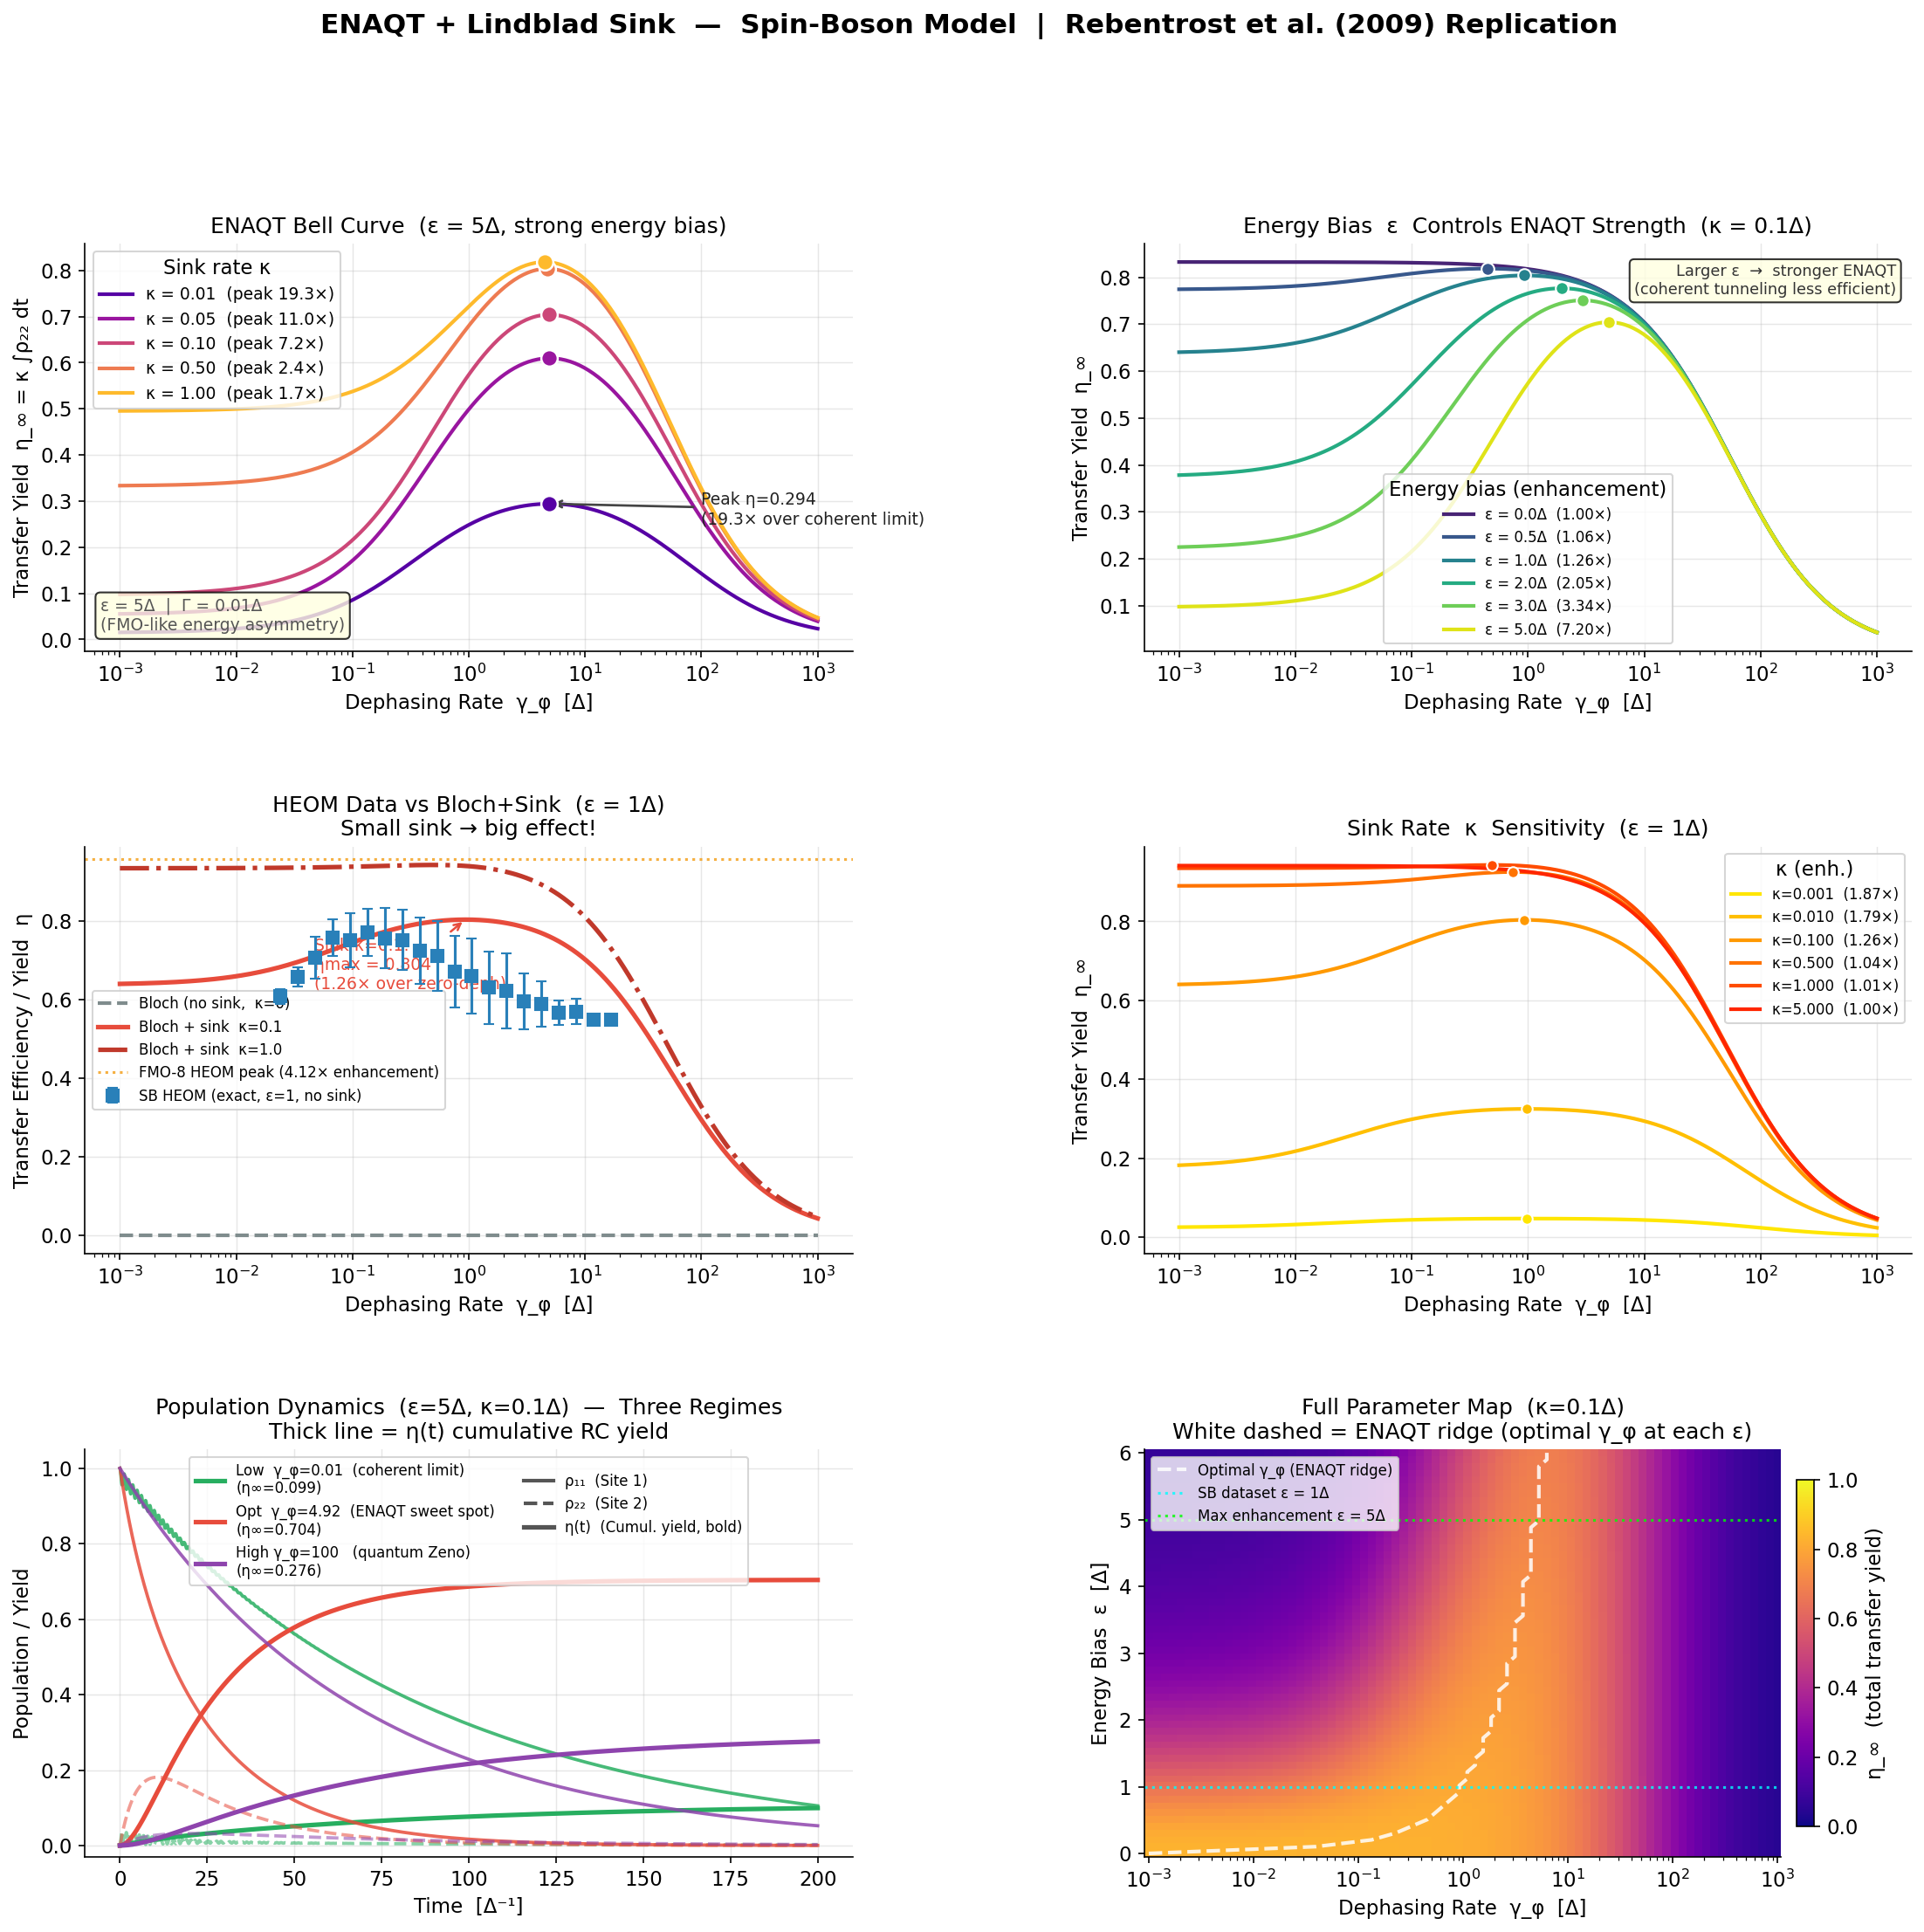
\includegraphics[width=\columnwidth]{enaqt_sb_sink.png}
\caption{\label{fig:eps_sweep}
  Analytical Lindblad yield $\eta_\infty$ vs.\ $\gp$ for five energy biases
  $\varepsilon \in \{0, 0.5, 1, 2, 5\}\Delta$ with sink $\kappa=0.1\Delta$
  ($N=2$, $\Gamma=0.01\Delta$).
  Enhancement grows from $1.06\times$ ($\varepsilon=0.5\Delta$) to $7.20\times$
  ($\varepsilon=5\Delta$).
  Inset: optimal $\gps$ scales linearly with $\varepsilon$.
}
\end{figure}

\begin{figure}[h]
\centering
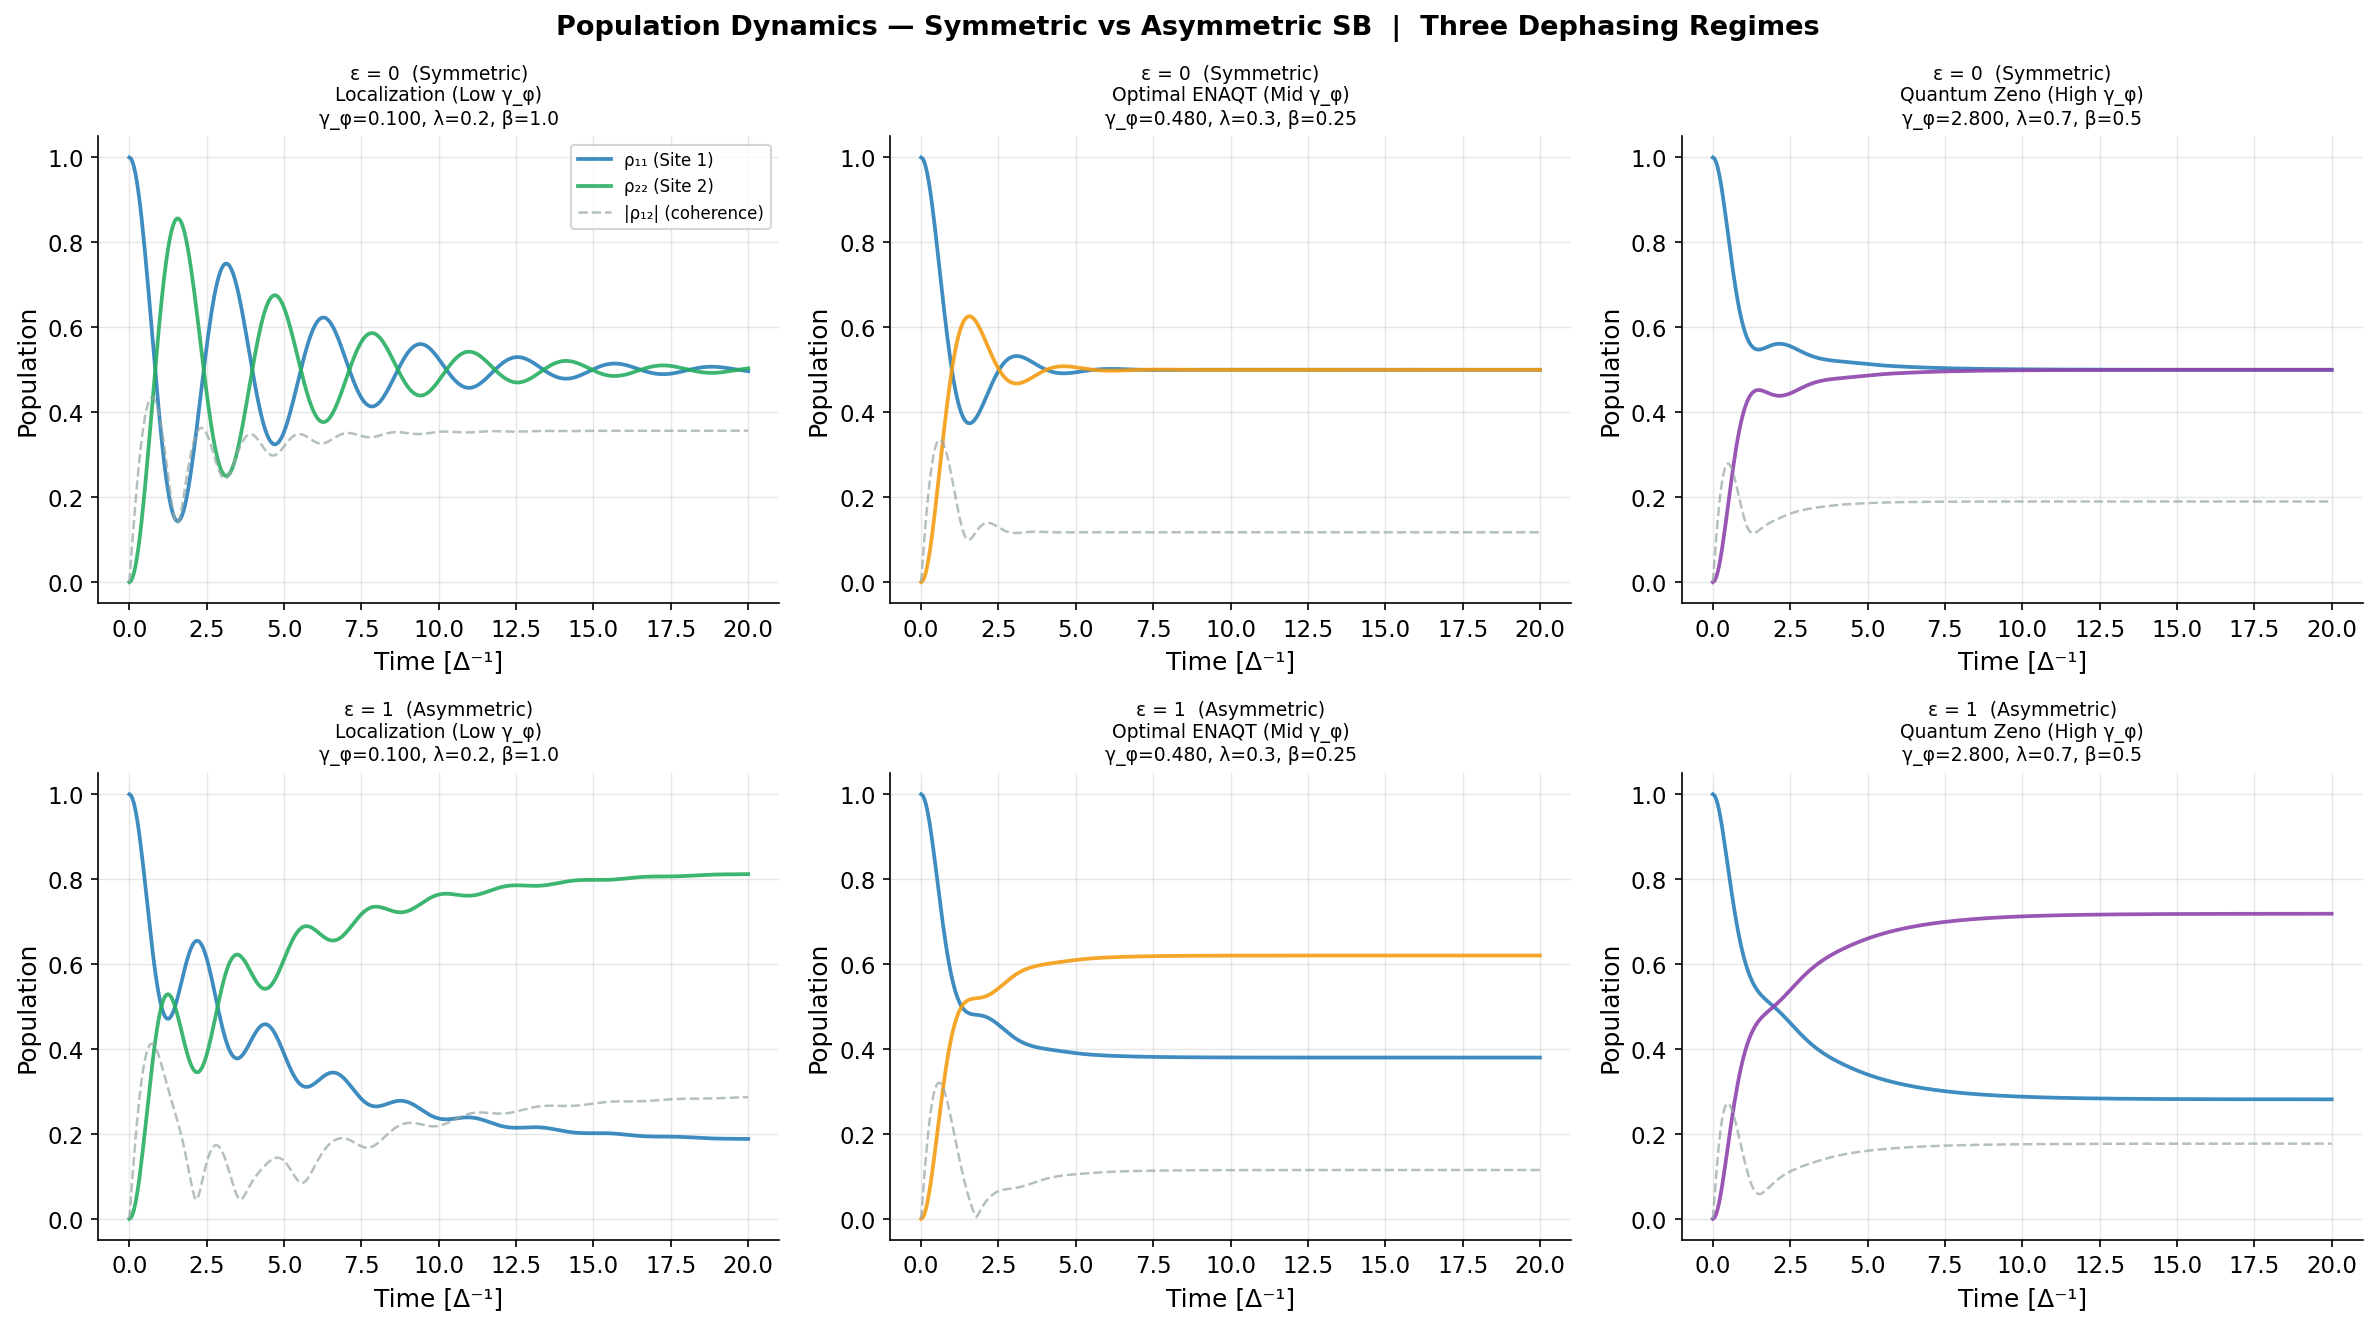
\includegraphics[width=\columnwidth]{enaqt_sb_dynamics_gallery.png}
\caption{\label{fig:gallery}
  Gallery of 12 representative HEOM spin-boson trajectories from QD3SET-1
  illustrating the three ENAQT regimes: persistent Rabi oscillations (low $\gp$),
  noise-damped rapid transfer (optimal $\gp$), and quantum Zeno freezing
  (high $\gp$).
  Color encodes cumulative transfer at $t = 20\,\Delta^{-1}$.
}
\end{figure}

\begin{figure}[h]
\centering
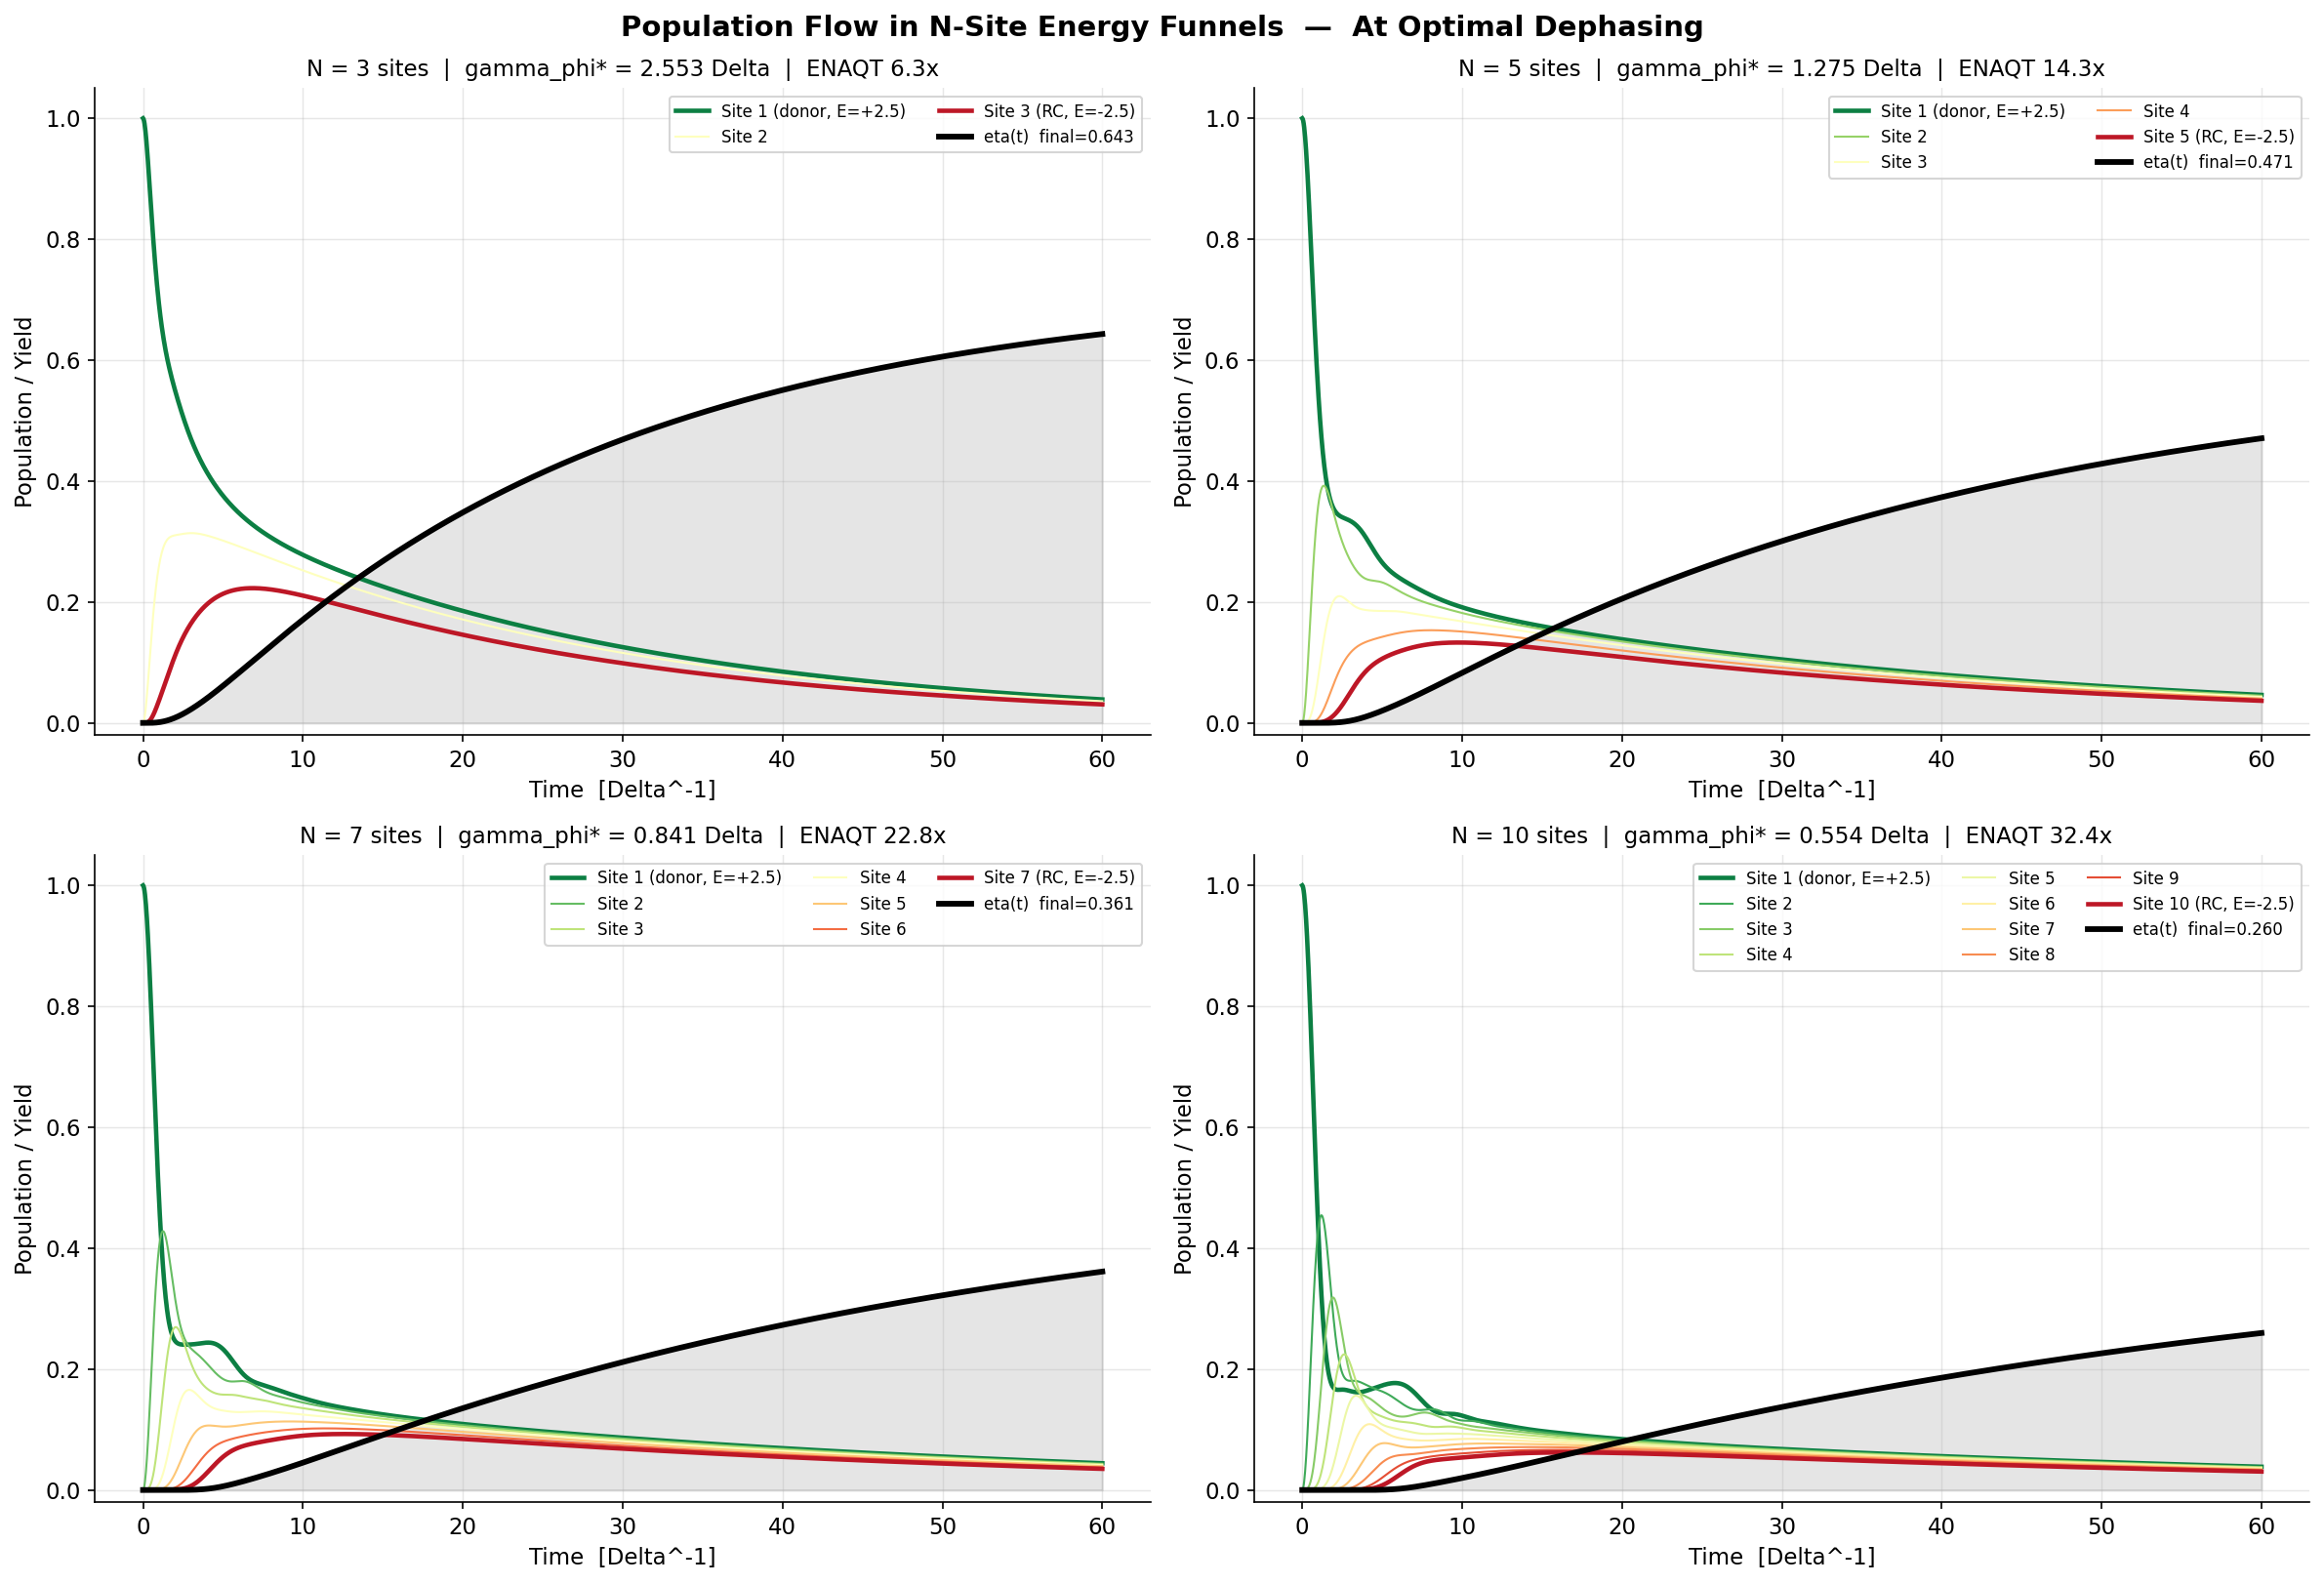
\includegraphics[width=\columnwidth]{enaqt_nsite_dynamics.png}
\caption{\label{fig:dynamics}
  Population dynamics at three dephasing regimes for $N=7$ energy funnel
  ($\varepsilon_\text{tot}=5\Delta$, $\kappa=0.1\Delta$, $\Gamma=0.01\Delta$).
  Panels show site populations $\rho_{jj}(t)$ and cumulative yield $\eta(t)$
  for coherent (low $\gp$), optimal ENAQT, and Zeno (high $\gp$) conditions.
}
\end{figure}

\begin{figure*}[h]
\centering
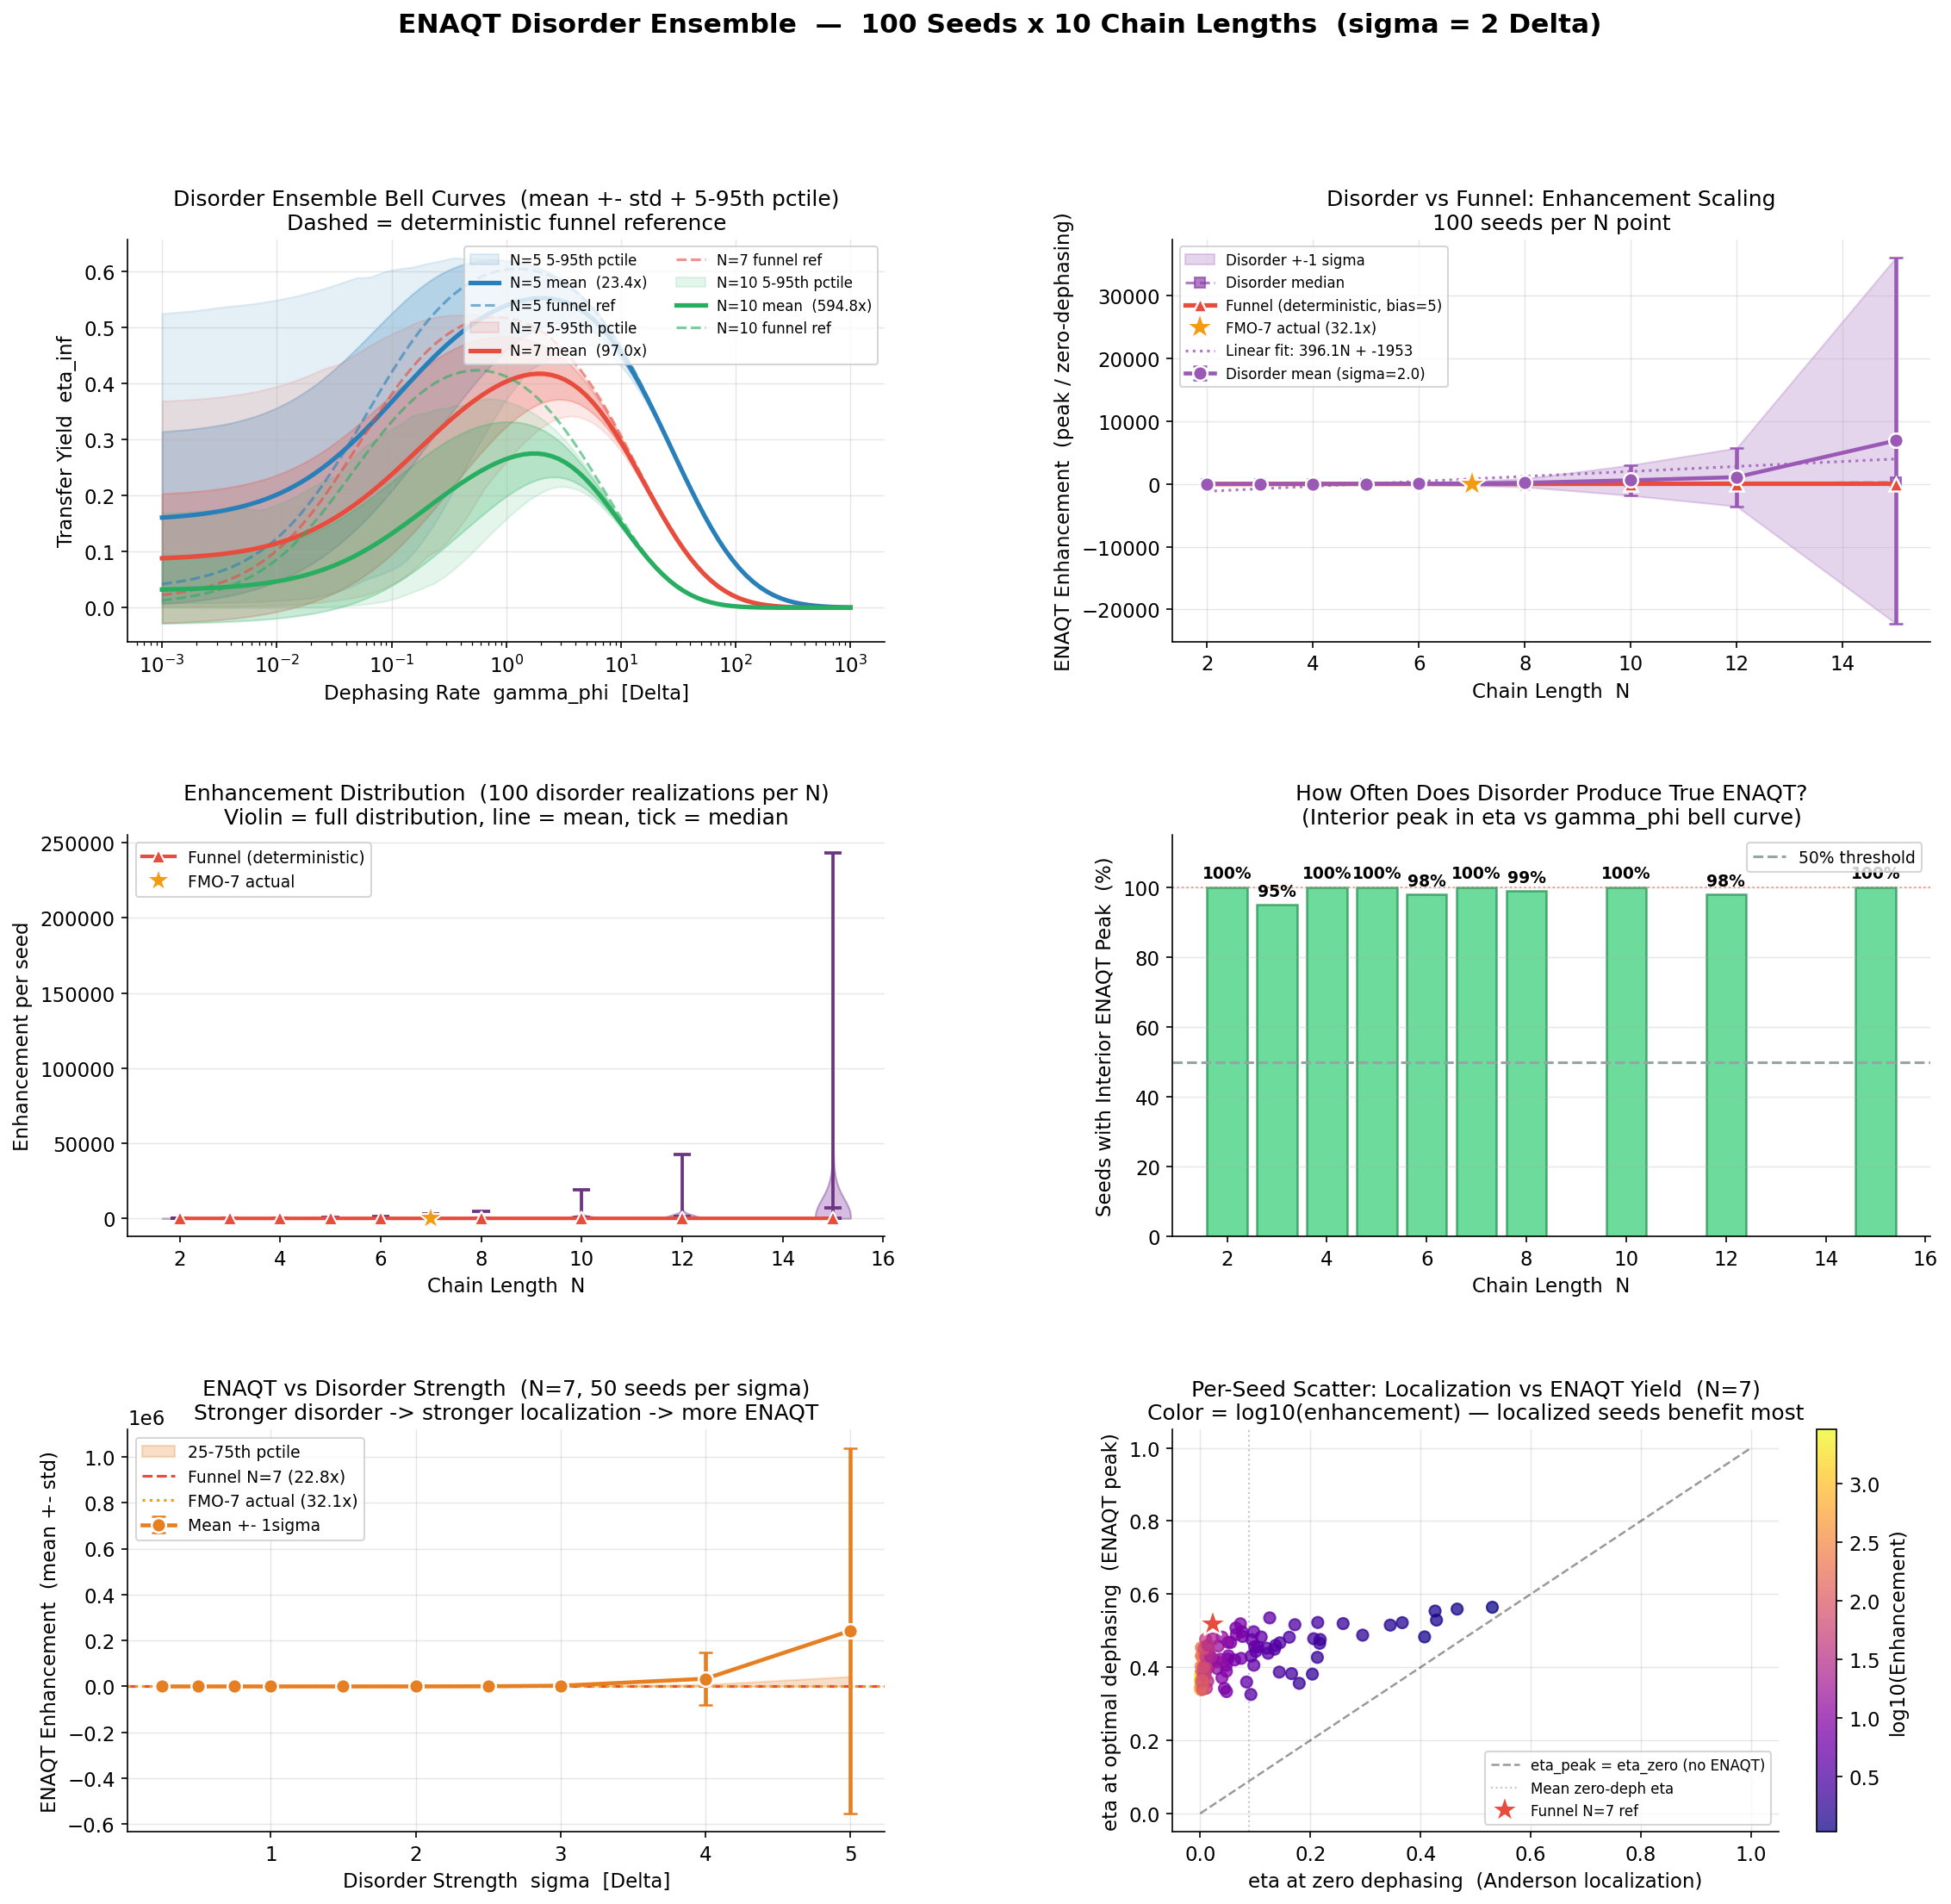
\includegraphics[width=\textwidth]{enaqt_disorder_ensemble.png}
\caption{\label{fig:disorder_full}
  Six-panel disorder ensemble summary (100 seeds, $\sigma=2\Delta$).
  (a) Violin plots of enhancement distributions vs.\ $N$; red line marks
      ordered-funnel reference.
  (b) Fraction of seeds showing a genuine interior ENAQT peak vs.\ $N$.
  (c) Median enhancement vs.\ $N$ for disordered (orange) and ordered funnel
      (blue).
  (d) Scatter of $\eta(\gp\to 0)$ vs.\ peak enhancement at $N=7$ and $N=15$,
      illustrating Anderson localization as the origin of the heavy tail.
  (e) Mean enhancement vs.\ $\sigma$ at $N=7$ (log-log scale).
  (f) Cumulative distribution of enhancement at $N=15$ showing the heavy
      right tail.
}
\end{figure*}

\end{document}
